% tEISguide.tex
% v4.0 released January 2014

\documentclass[]{tEIS2e}

\usepackage{float}
\usepackage{subfigure}
\usepackage{amssymb,amsmath,amsfonts}
\usepackage{color}
\usepackage{url}
\usepackage{graphicx}
\usepackage{multirow}
\usepackage{tabulary}

\usepackage{tikz}
\usetikzlibrary{positioning}
\usepackage[percent]{overpic}

\usepackage{listings} 
\lstset{
    breaklines=true,
    basicstyle=\ttfamily\scriptsize,
    columns=flexible,
}

\usepackage[pdftex,pdfpagelabels,bookmarks,hyperindex,hyperfigures]{hyperref}
\usepackage[nogroupskip,automake,nonumberlist,nopostdot,shortcuts,section]{glossaries}

\mathchardef\mhyphen="2D % Define a "math hyphen"
\graphicspath{{../../Figures/}}
%% myFigures.tex
% A common file to store all figure definitions
%
% In preparing your thesis, one of the first things you should do is
% organize your figures.  Then, one of the last things you'll do is
% reorder your figures so they display where you want them to in the
% text.  Organizing figure definitions in a common files helps:
%
%   1. Write new figures using earlier examples.
%
%   2.  Isolate code and minimize the risk of introducing bugs in the
%   final editing process.  Trust me, moving around just one line of
%   code is easier.
%
%   3.  Reuse figures in other papers.  <=== the best reason!
%
% Note command names can not include numbers and special characters.
%
% To make the file more searchable, use naming conventions that map
% the graphics filename labSetup.jpg to the command name \figlabSetup to the
% figure label fig:labSetup.
% 

\newcommand{\figproactiveFaultManagement}[1]{\begin{figure}
 \begin{center}
    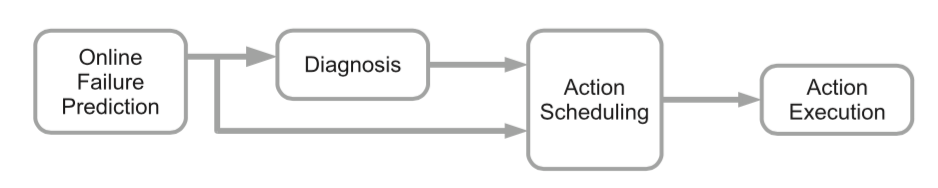
\includegraphics[width=#1]{proactiveFaultManagement}
     \caption[Proactive Fault Management~\cite{salfnerSurvey}]{The stages of
     proactive fault management~\cite{salfnerSurvey}.}
     \label{fig:proactiveFaultManagement}
 \end{center}
\end{figure}
}

\newcommand{\figonlinePrediction}[1]{\begin{figure}
 \begin{center}
    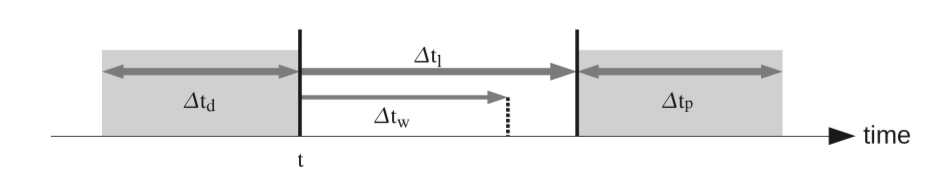
\includegraphics[width=#1]{onlinePrediction}
     \caption[\ac{OFP}~\cite{salfnerSurvey}]{The timeline for
     \ac{OFP}~\cite{salfnerSurvey}.}
     \label{fig:onlinePrediction}
 \end{center}
\end{figure}
}

\newcommand{\figfailureFlowDiagram}[1]{\begin{figure}
 \begin{center}
    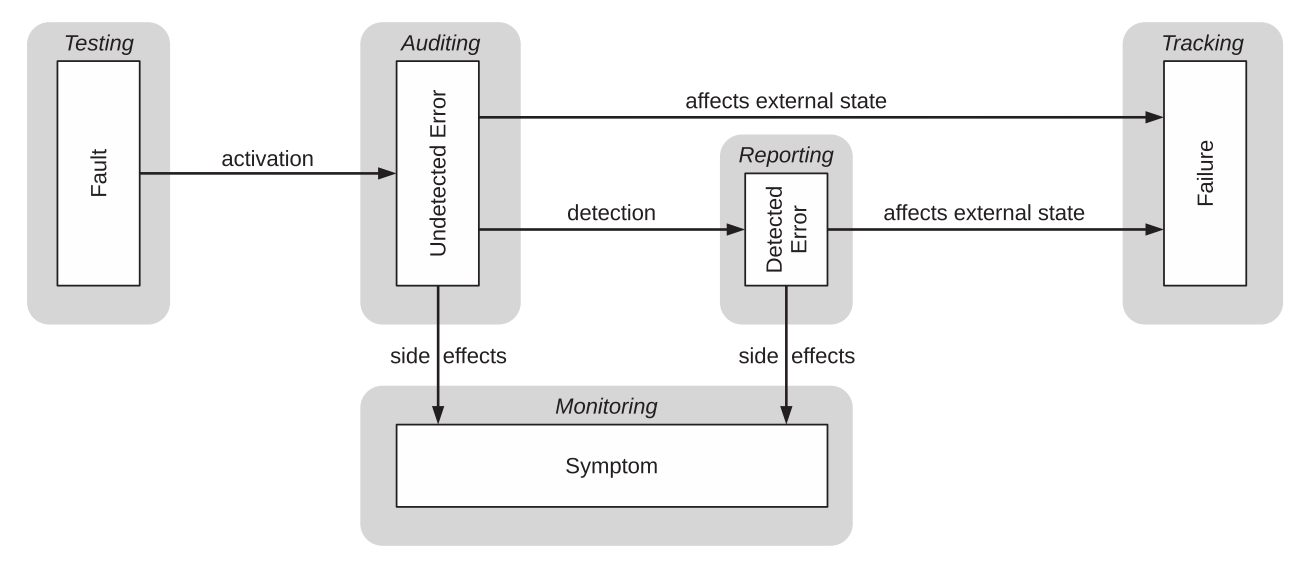
\includegraphics[width=#1]{failureFlowDiagram}
     \caption[Failure Flow Diagram~\cite{salfnerSurvey}]{How faults and errors
     evolve into failure with the associated methods for detection represented
     by enclosing gray boxes~\cite{salfnerSurvey}.}
     \label{fig:failureFlowDiagram}
 \end{center}
 %\vspace{-0.2 in}
\end{figure}
}

\newcommand{\figROC}[1]{\begin{figure}
 \begin{center}
    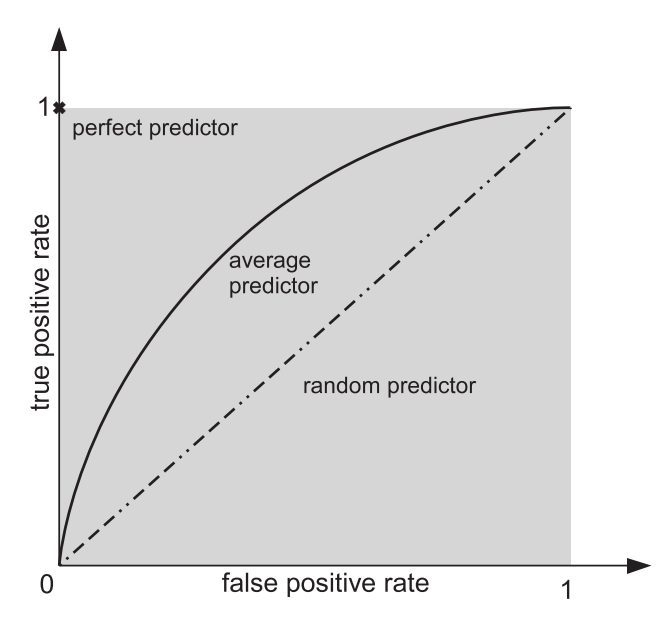
\includegraphics[width=#1]{ROC}
     \caption[Sample \ac{ROC} Plots~\cite{salfnerSurvey}]{\ac{ROC} plots of
     perfect, average, and random predictors~\cite{salfnerSurvey}.}
     \label{fig:ROC}
 \end{center}
\end{figure}
}

\newcommand{\figprecisionRecallCurve}[1]{\begin{figure}
 \begin{center}
    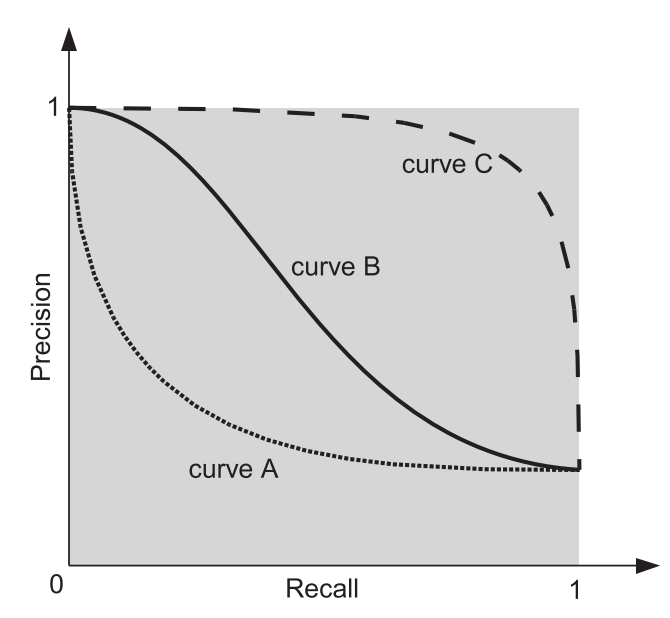
\includegraphics[width=#1]{precisionRecallCurve}
     \caption[Sample Precision/Recall Curves~\cite{salfnerSurvey}]{Sample
     precision/recall curves~\cite{salfnerSurvey}.  Curve $A$ represents a
     poorly performing predictor, curve $B$ an average predictor, and curve $C$
     an exceptional predictor.}
     \label{fig:precisionRecallCurve}
 \end{center}
\end{figure}
}

\newcommand{\figpatternRecognition}[1]{\begin{figure}
 \begin{center}
    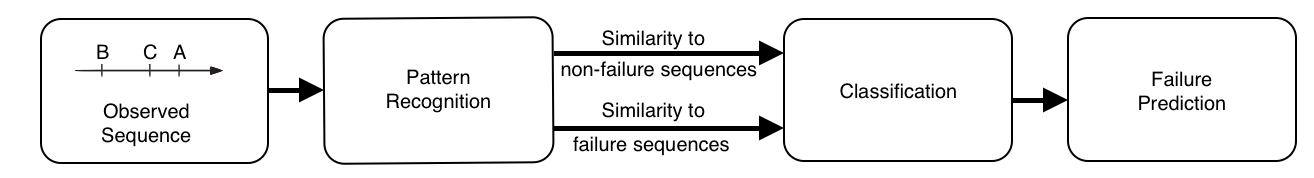
\includegraphics[width=#1]{patternRecognition}
     \caption[Pattern recognition in reported errors~\cite{salfnerSurvey}]{How
     pattern recognition is accomplished in reported
     errors~\cite{salfnerSurvey}.}
     \label{fig:patternRecognition}
 \end{center}
\end{figure}
}

\newcommand{\figAFP}[1]{\begin{figure}[t!h]
 \begin{center}
    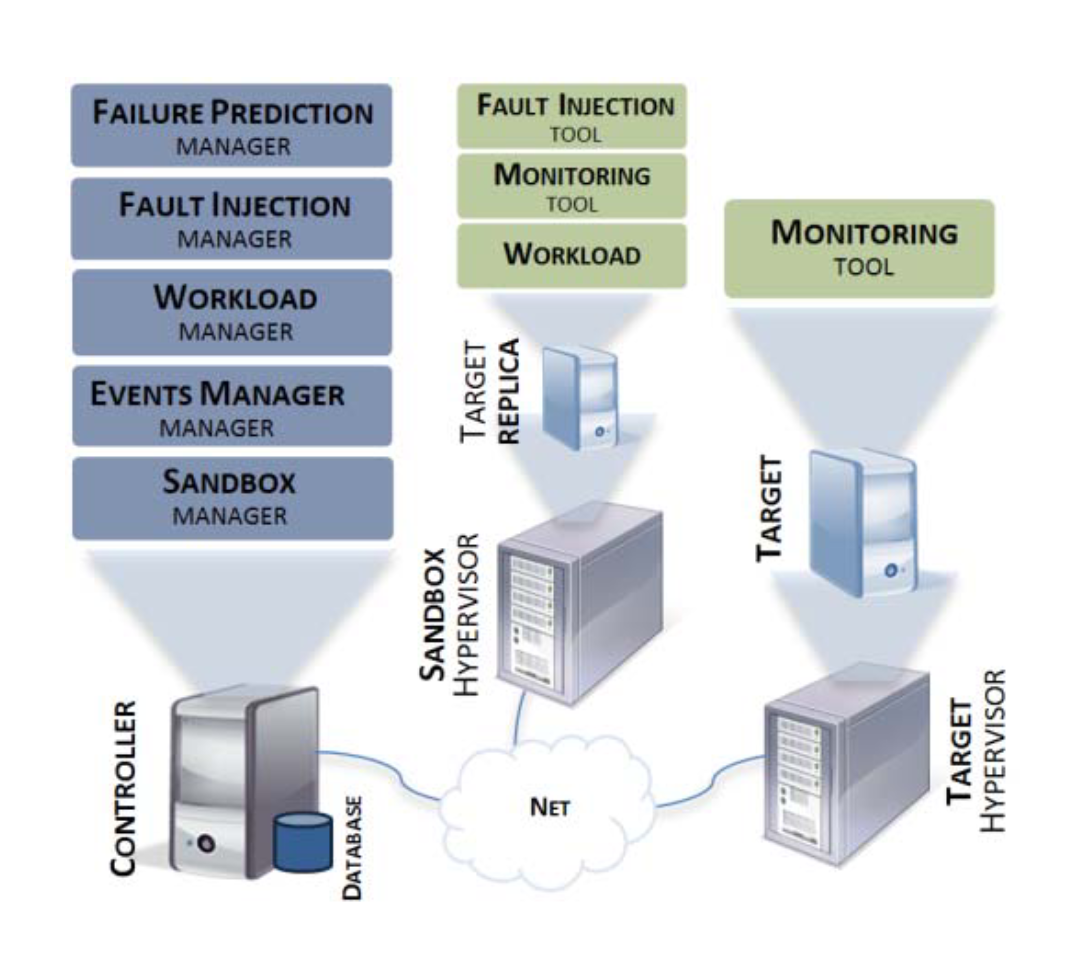
\includegraphics[width=#1]{AFP}
     \caption{The \ac{AFP} framework~\cite{irrera2015}.}
     \label{fig:AFP}
 \end{center}
\end{figure}
}

\definecolor{airforceblue}{rgb}{0.36, 0.54, 0.66}
\definecolor{armygreen}{rgb}{0.29, 0.33, 0.13}

\newcommand{\figannotatedAFPcolor}{\begin{figure}
 \begin{center}
     \begin{overpic}[width=5in,scale=.25]{annotatedAFPcolor}
       \put(8,0){
         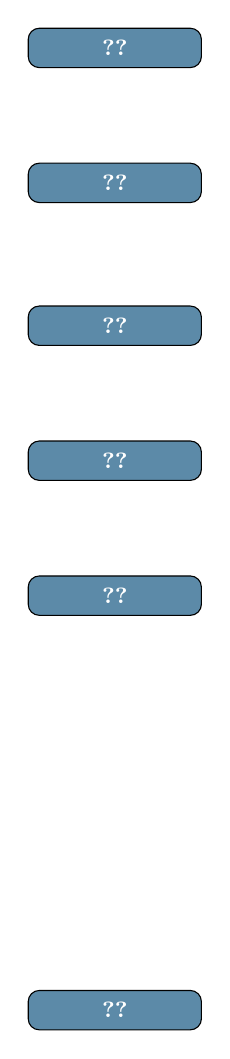
\begin{tikzpicture}
           [node font=\footnotesize, label/.style={rectangle, draw,
           fill=airforceblue, text width=2cm, text badly centered, minimum
           height=0.5cm, rounded corners}]

           \node[label] (FPMgr)
             {\textcolor{white}{\ref{sec:failurePrediction}}};
           \node[label, below=1.2cm of FPMgr] (FIMgr) 
             {\textcolor{white}{\ref{sec:faultInjectionMgr}}};
           \node[label, below=1.3cm of FIMgr] (WMgr) 
             {\textcolor{white}{\ref{sec:workloadMgr}}};
           \node[label, below=1.2cm of WMgr] (EMMgr) 
             {\textcolor{white}{\ref{sec:eventsManagerMgr}}};
           \node[label, below=1.2cm of EMMgr] (SMgr) 
             {\textcolor{white}{\ref{sec:sandboxMgr}}};
           \node[label, below=4.75cm of SMgr] (Controller) 
             {\textcolor{white}{\ref{sec:controller}}};
         \end{tikzpicture}
       }

       \put(40,60.5){
         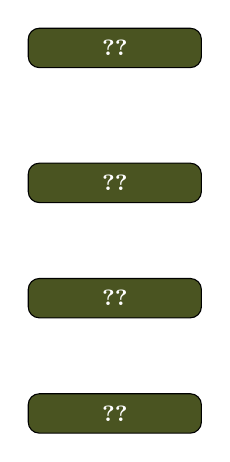
\begin{tikzpicture}
           [node font=\footnotesize, label/.style={rectangle, draw,
           fill=armygreen, text width=2cm, text badly centered, minimum
           height=0.5cm, rounded corners}]

           \node[label] (Sandbox)
             {\textcolor{white}{\ref{sec:sandbox}}};
           \node[label, below=1.2cm of Sandbox] (SBFITool)
             {\textcolor{white}{\ref{sec:faultInjectionTool}}};
           \node[label, below=0.95cm of SBFITool] (SBMTool) 
             {\textcolor{white}{\ref{sec:sandboxMonitoringTool}}};
           \node[label, below=0.95cm of SBMTool] (SBWorkload) 
             {\textcolor{white}{\ref{sec:sandboxWorkload}}};
         \end{tikzpicture}
       }

       \put(66,0){
         
\begin{tikzpicture}
           [node font=\footnotesize, label/.style={rectangle, draw,
           fill=armygreen, text width=2cm, text badly centered, minimum
           height=0.5cm, rounded corners}]

           \node[label] (MonTool)
             {\textcolor{white}{\ref{sec:targetMonitoringTool}}};
           \node[label, below=7.85cm of MonTool] (Target)
             {\textcolor{white}{\ref{sec:target}}};
         \end{tikzpicture}
       }
     \end{overpic}
     \caption[Annotated \ac{AFP} Framework~\cite{irrera2015}]{The \ac{AFP}
     framework implementation~\cite{irrera2015} with modified components
     highlighted.}
     \label{fig:annotatedAFP}
 \end{center}
\end{figure}
}

\newcommand{\figannotatedAFP}{\begin{figure}
 \begin{center}
     \begin{overpic}[width=5in,scale=.25]{annotatedAFP}
       \put(8,0){
         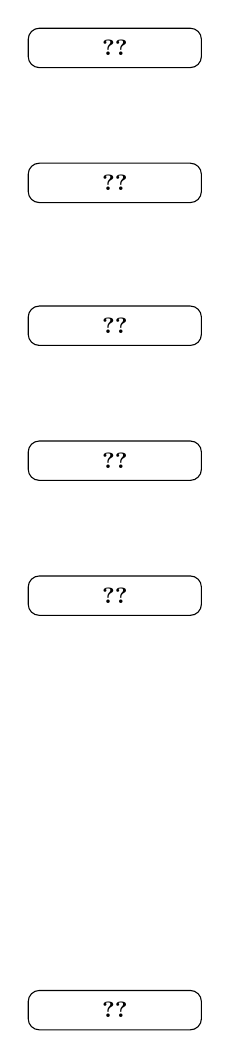
\begin{tikzpicture}
           [node font=\footnotesize, label/.style={rectangle, draw,
           fill=white, text width=2cm, text badly centered, minimum
           height=0.5cm, rounded corners}]

           \node[label] (FPMgr)
             {\textcolor{black}{\ref{sec:failurePrediction}}};
           \node[label, below=1.2cm of FPMgr] (FIMgr) 
             {\textcolor{black}{\ref{sec:faultInjectionMgr}}};
           \node[label, below=1.3cm of FIMgr] (WMgr) 
             {\textcolor{black}{\ref{sec:workloadMgr}}};
           \node[label, below=1.2cm of WMgr] (EMMgr) 
             {\textcolor{black}{\ref{sec:eventsManagerMgr}}};
           \node[label, below=1.2cm of EMMgr] (SMgr) 
             {\textcolor{black}{\ref{sec:sandboxMgr}}};
           \node[label, below=4.75cm of SMgr] (Controller) 
             {\textcolor{black}{\ref{sec:controller}}};
         \end{tikzpicture}
       }

       \put(40,60.5){
         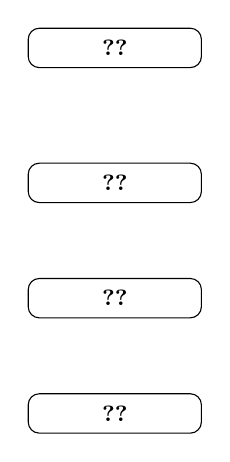
\begin{tikzpicture}
           [node font=\footnotesize, label/.style={rectangle, draw,
           fill=white, text width=2cm, text badly centered, minimum
           height=0.5cm, rounded corners}]

           \node[label] (Sandbox)
             {\textcolor{black}{\ref{sec:sandbox}}};
           \node[label, below=1.2cm of Sandbox] (SBFITool)
             {\textcolor{black}{\ref{sec:faultInjectionTool}}};
           \node[label, below=0.95cm of SBFITool] (SBMTool) 
             {\textcolor{black}{\ref{sec:sandboxMonitoringTool}}};
           \node[label, below=0.95cm of SBMTool] (SBWorkload) 
             {\textcolor{black}{\ref{sec:sandboxWorkload}}};
         \end{tikzpicture}
       }

       \put(66,0){
         \begin{tikzpicture}
           [node font=\footnotesize, label/.style={rectangle, draw,
           fill=white, text width=2cm, text badly centered, minimum
           height=0.5cm, rounded corners}]

           \node[label] (MonTool)
             {\textcolor{black}{\ref{sec:targetMonitoringTool}}};
           \node[label, below=7.85cm of MonTool] (Target)
             {\textcolor{black}{\ref{sec:target}}};
         \end{tikzpicture}
       }
     \end{overpic}
     \caption[Annotated \ac{AFP} Framework~\cite{irrera2015}]{The \ac{AFP}
     framework implementation~\cite{irrera2015} with modified components
     highlighted.}
     \label{fig:annotatedAFP}
 \end{center}
\end{figure}
}

\newcommand{\figTrainingPhase}[1]{\begin{figure}[h!t]
 \begin{center}
  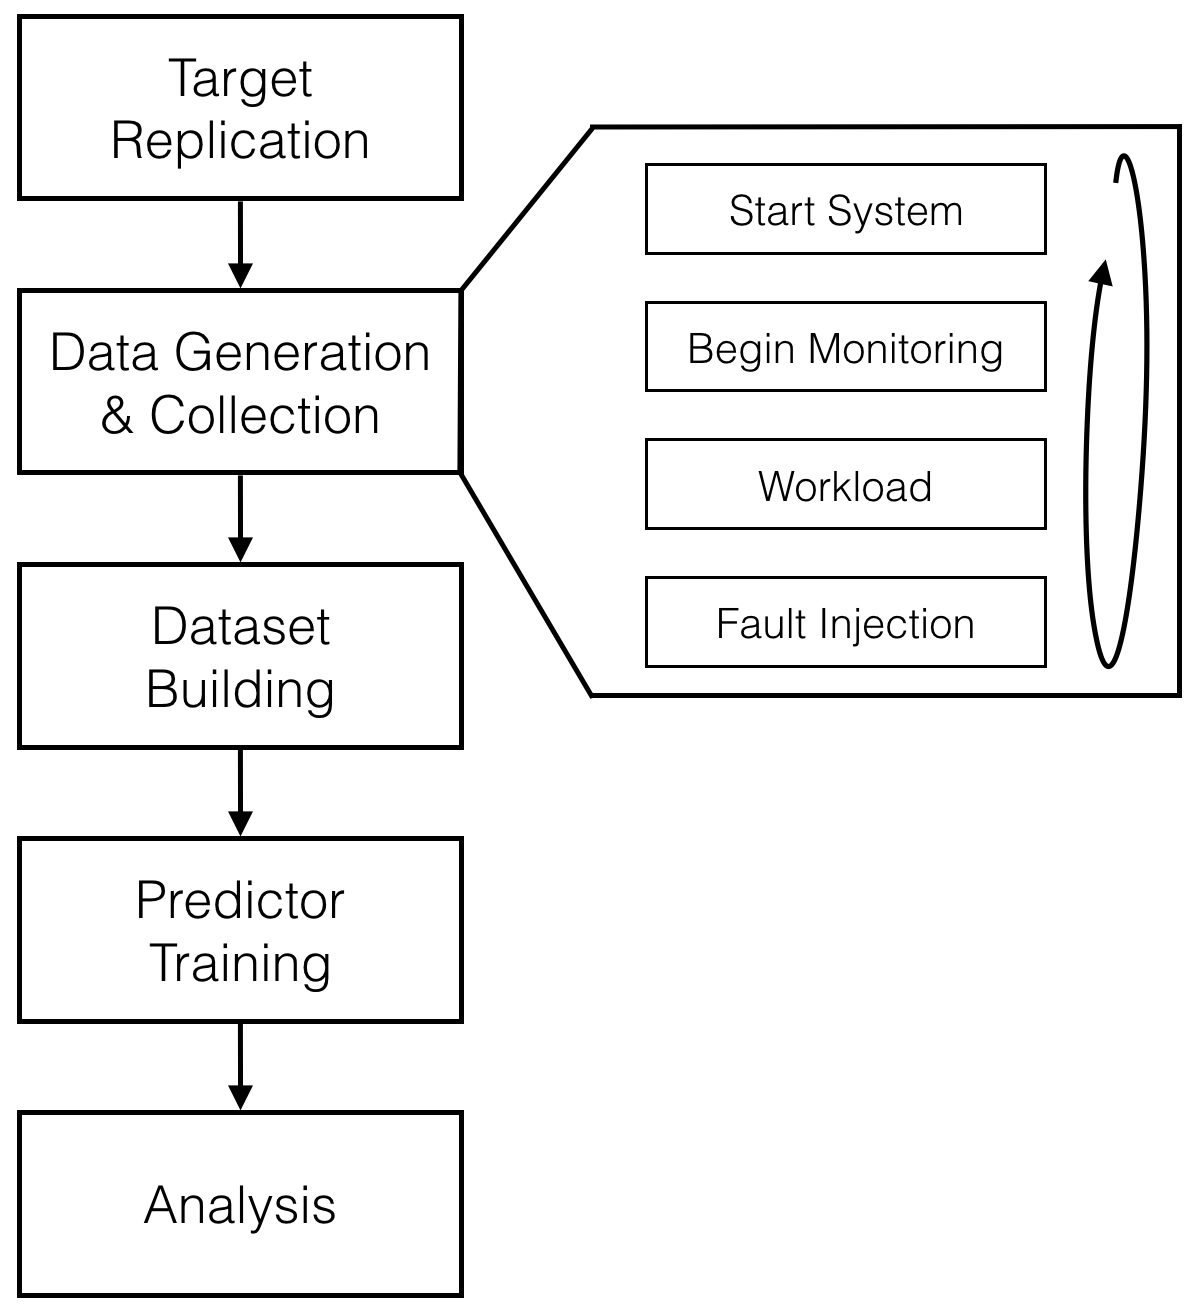
\includegraphics[width=#1]{TrainingPhase}
  \caption[\ac{AFP} Training Phase~\cite{irrera2015}]{The flow of the major
  steps involved in the \ac{AFP} framework training phase~\cite{irrera2015}.}
  \label{fig:TrainingPhase}
 \end{center}
\end{figure}
}

\newcommand{\figExecutionPhase}[1]{\begin{figure}[h!t]
  \begin{center}
    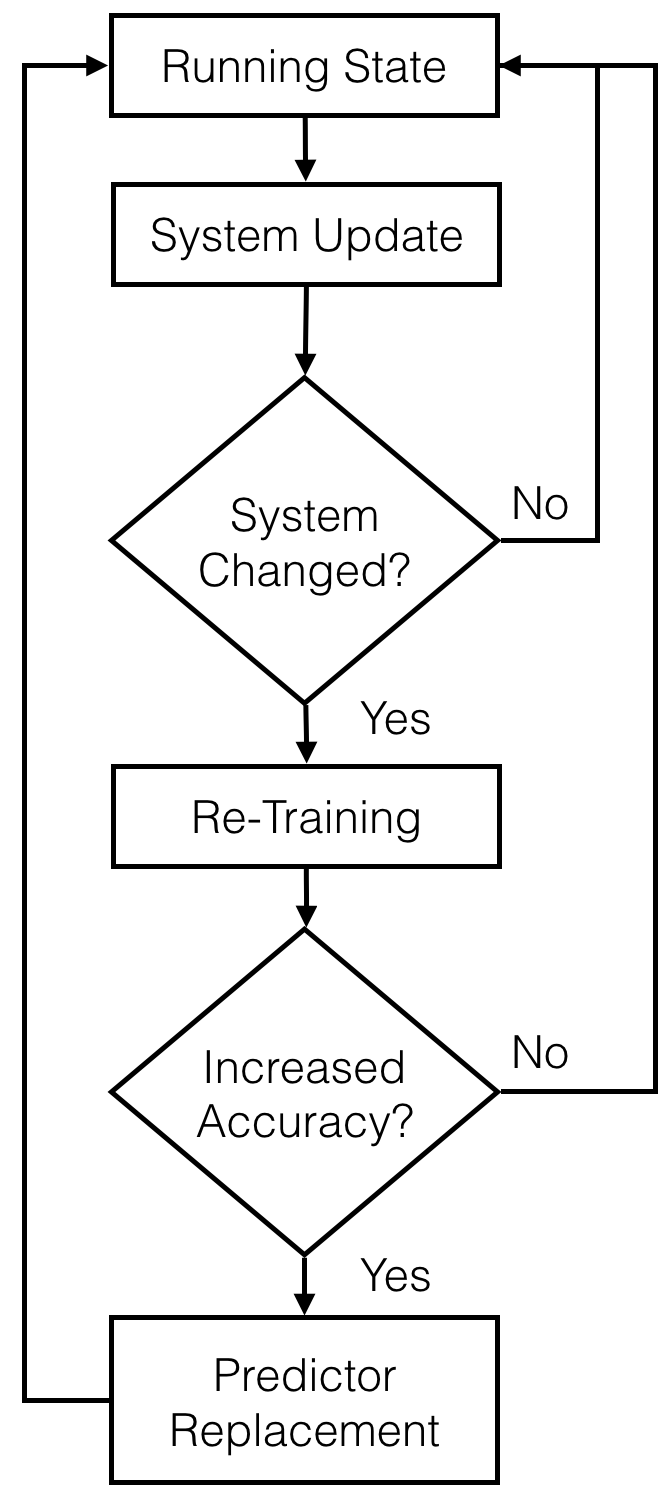
\includegraphics[width=#1]{ExecutionPhase}
    \caption[\ac{AFP} Execution Phase~\cite{irrera2015}]{The flow of the major
    steps involved in the \ac{AFP} framework execution
    phase~\cite{irrera2015}.}
    \label{fig:ExecutionPhase}
  \end{center}
\end{figure}
}


\newcommand{\figExecutionPhaseHoriz}[1]{\begin{figure}
  \begin{center}
    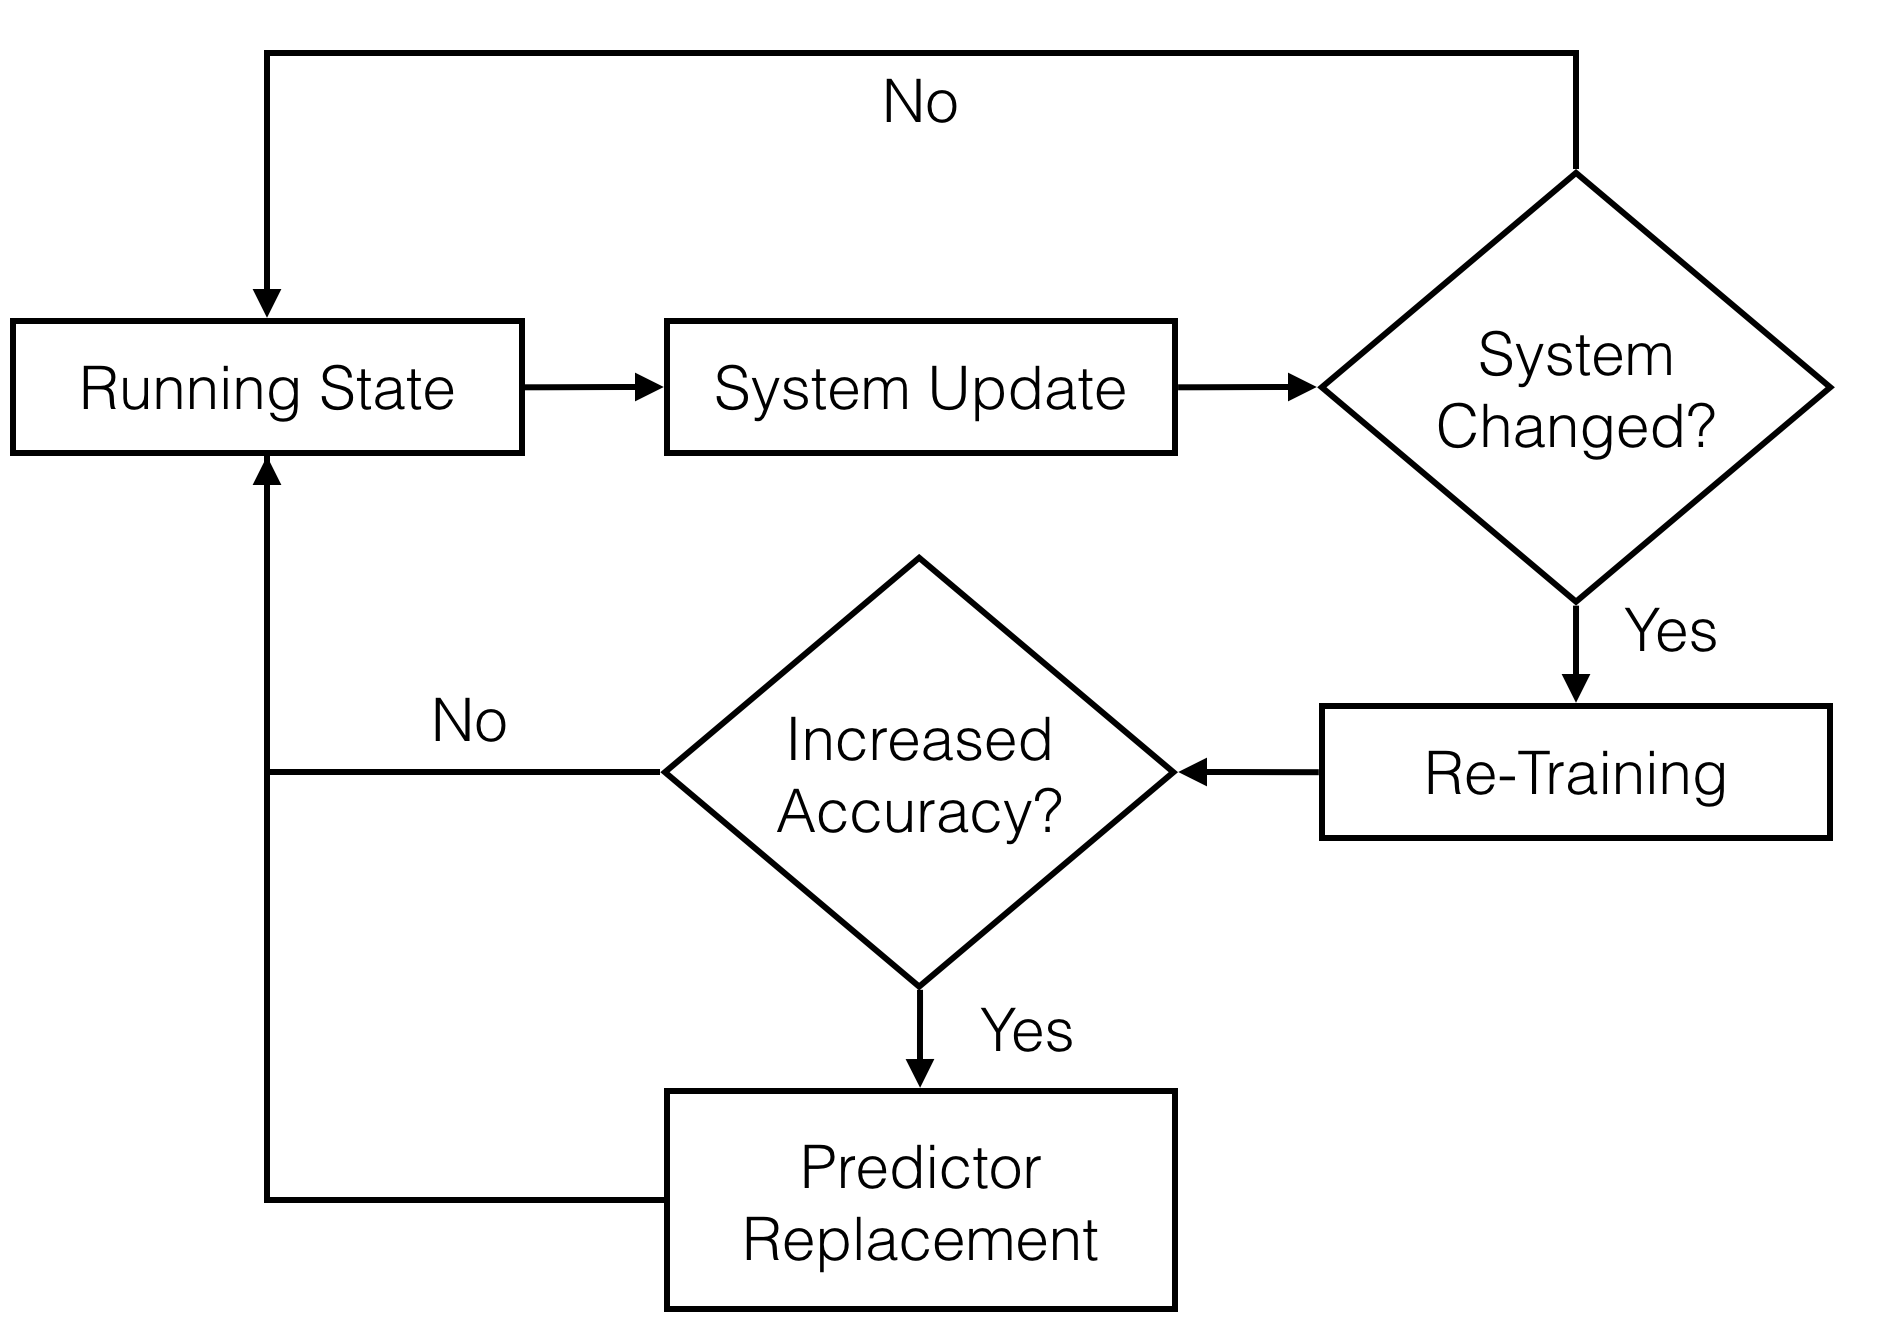
\includegraphics[width=#1]{ExecutionPhaseHoriz}
    \caption[\ac{AFP} Execution Phase~\cite{irrera2015}]{The flow of the major
    steps involved in the \ac{AFP} framework execution
    phase~\cite{irrera2015}.}
    \label{fig:ExecutionPhaseHoriz}
  \end{center}
\end{figure}
}

\newcommand{\figAuthDCPPS}[1]{\begin{figure}
 \begin{center}
  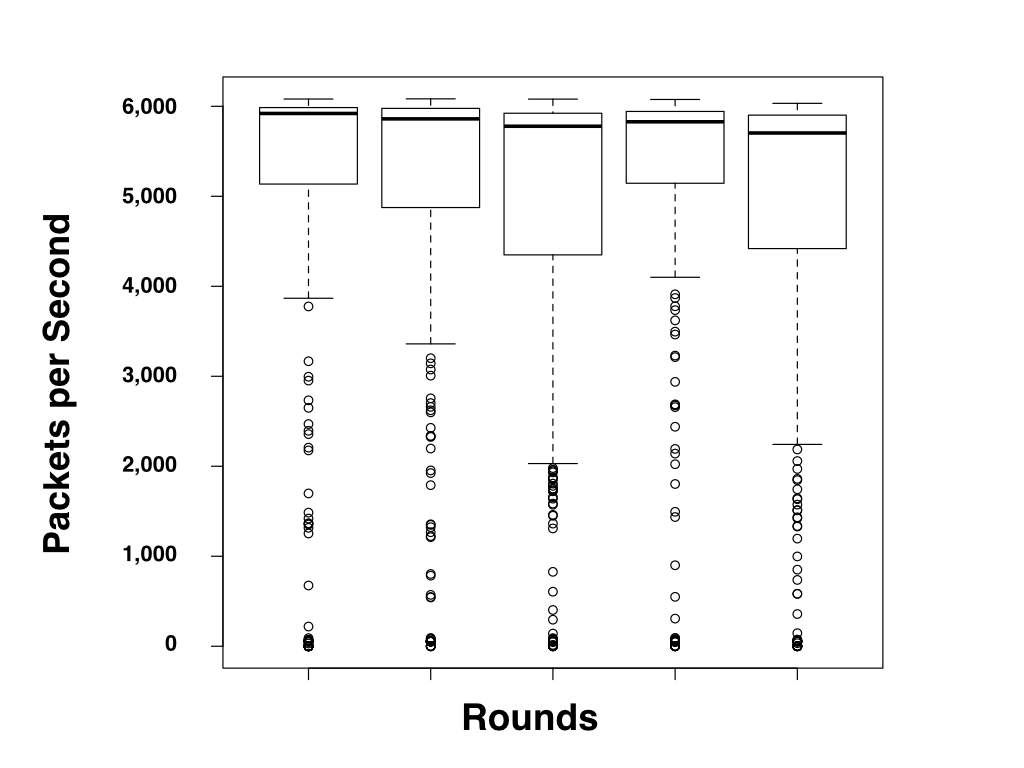
\includegraphics[width=#1]{DPLG/authDCPPS}
  \caption[Domain Controller Packets per Second]{How many packets per second
  were sent or received by the domain controller across all five rounds of the
  first test.  In each test, we captured approximately 1.8 million packets.}
  \label{fig:authDCPPS}
 \end{center}
\end{figure}
}

\newcommand{\figAuthClientPPS}[1]{\begin{figure}
 \begin{center}
  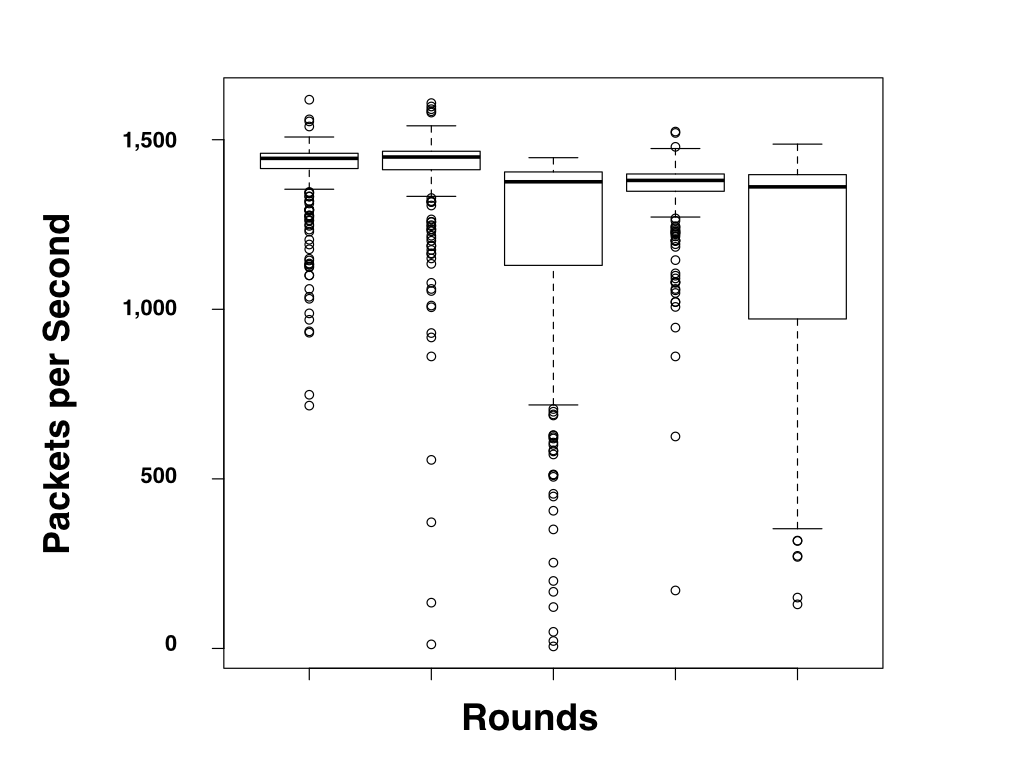
\includegraphics[width=#1]{DPLG/authClientPPS}
  \caption[Client Packets per Second]{How many packets per second were sent or
  received by one of the clients across all five rounds of the first test.}
  \label{fig:authClientPPS}
 \end{center}
\end{figure}
}

\newcommand{\figAuthDCMetrics}[1]{\begin{figure}
 \begin{center}
  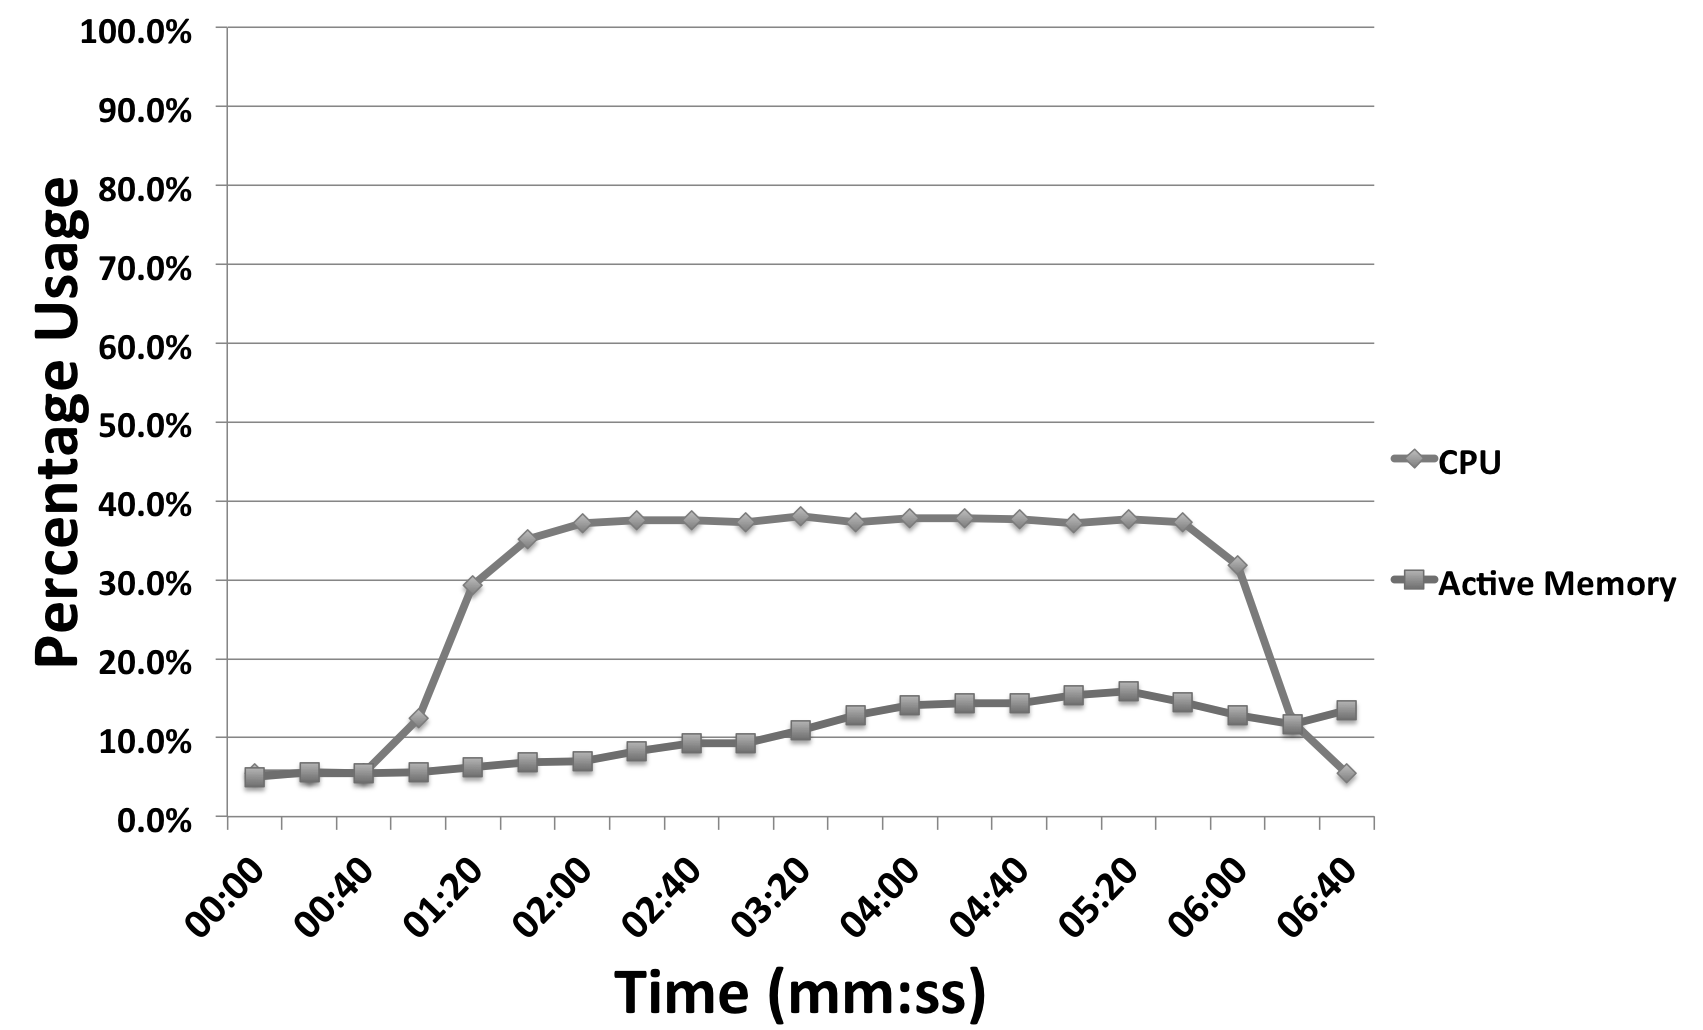
\includegraphics[width=#1]{DPLG/authDCMetrics}
  \caption[Test 1:  Domain Controller Performance]{Domain controller CPU and
  memory utilization during the first test.}
  \label{fig:authDCMetrics}
 \end{center}
\end{figure}
}

\newcommand{\figOFPTaxonomy}[1]{\begin{figure}
 \begin{center}
  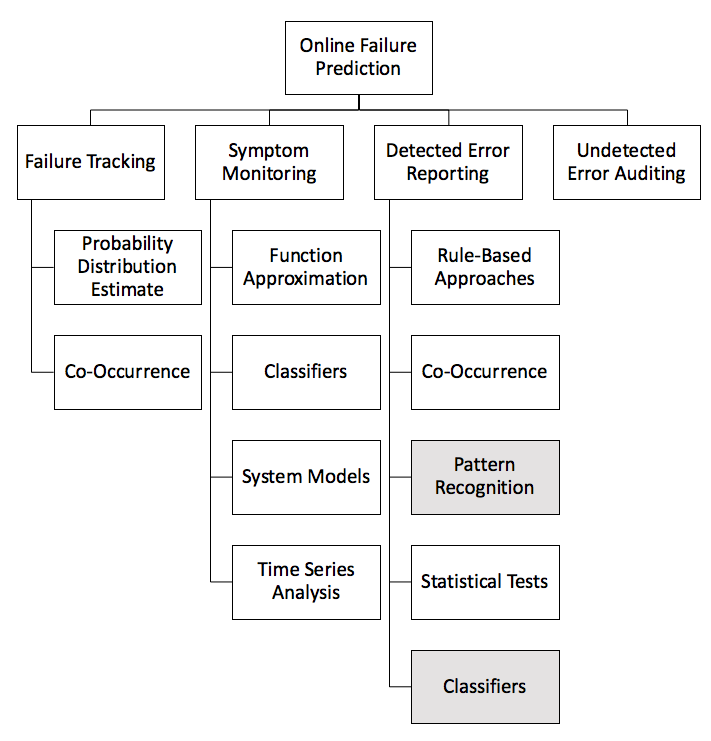
\includegraphics[width=#1]{OFPTaxonomy}
  \caption[Taxonomy of \ac{OFP} Approaches]{Taxonomy of approaches to online
  failure prediction~\cite{salfnerSurvey}.  The two categories into which this
  research falls are highlighted.}
  \label{fig:OFPTaxonomy}
 \end{center}
\end{figure}
}

\newcommand{\figMemLeakROC}[1]{\begin{figure}
 \begin{center}
  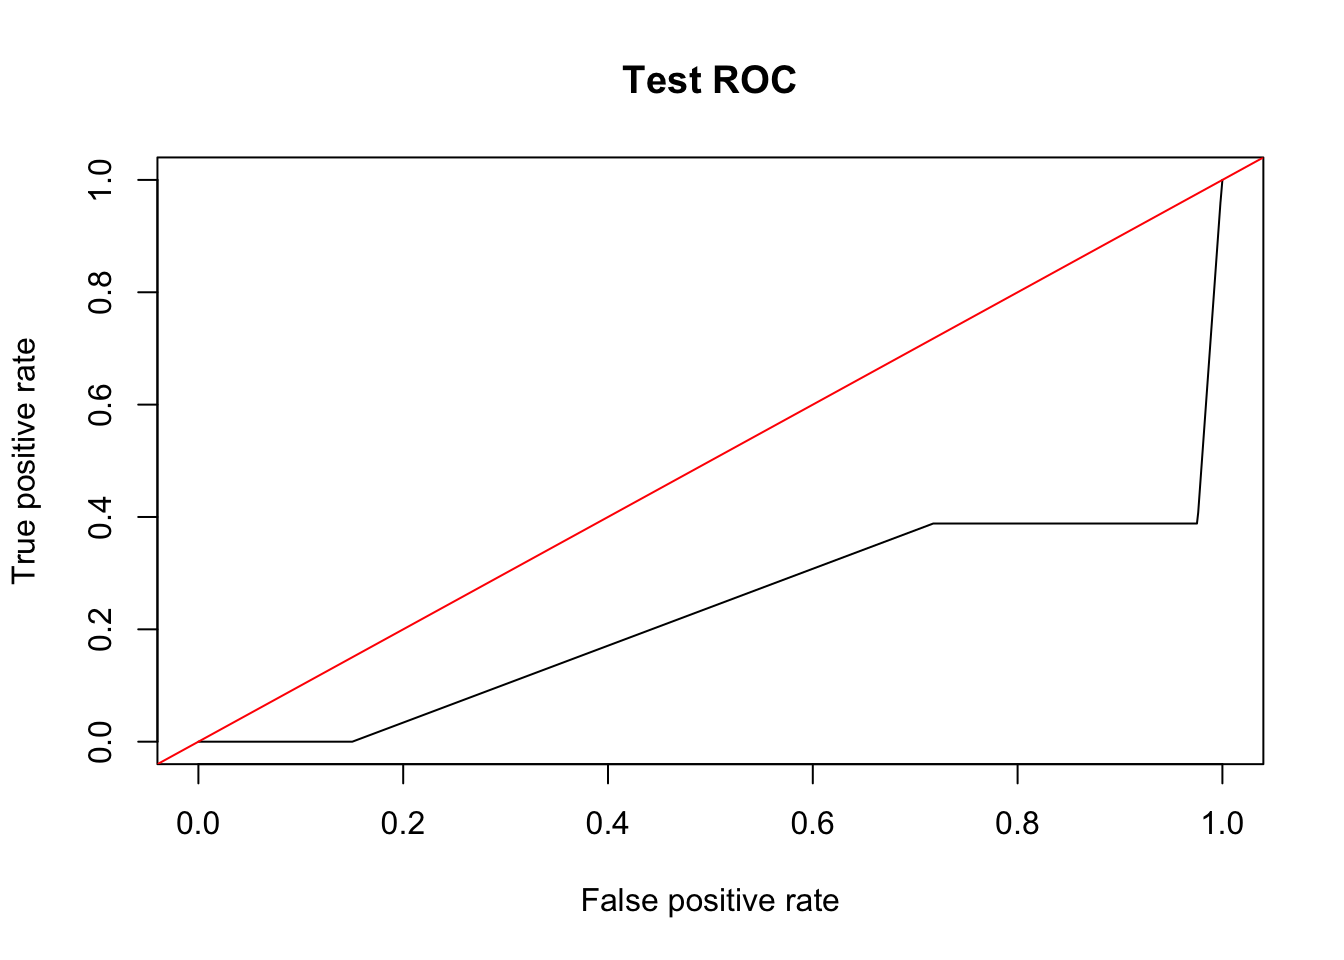
\includegraphics[width=#1]{MemLeakROC}
  \caption[\ac{SVM} Memory Leak \ac{ROC} Curve]{\ac{SVM} memory leak test data
  \ac{ROC} curve.}
  \label{fig:memLeakROC}
 \end{center}
\end{figure}
}

\newcommand{\figMemLeakCompare}[1]{\begin{figure}
 \begin{center}
  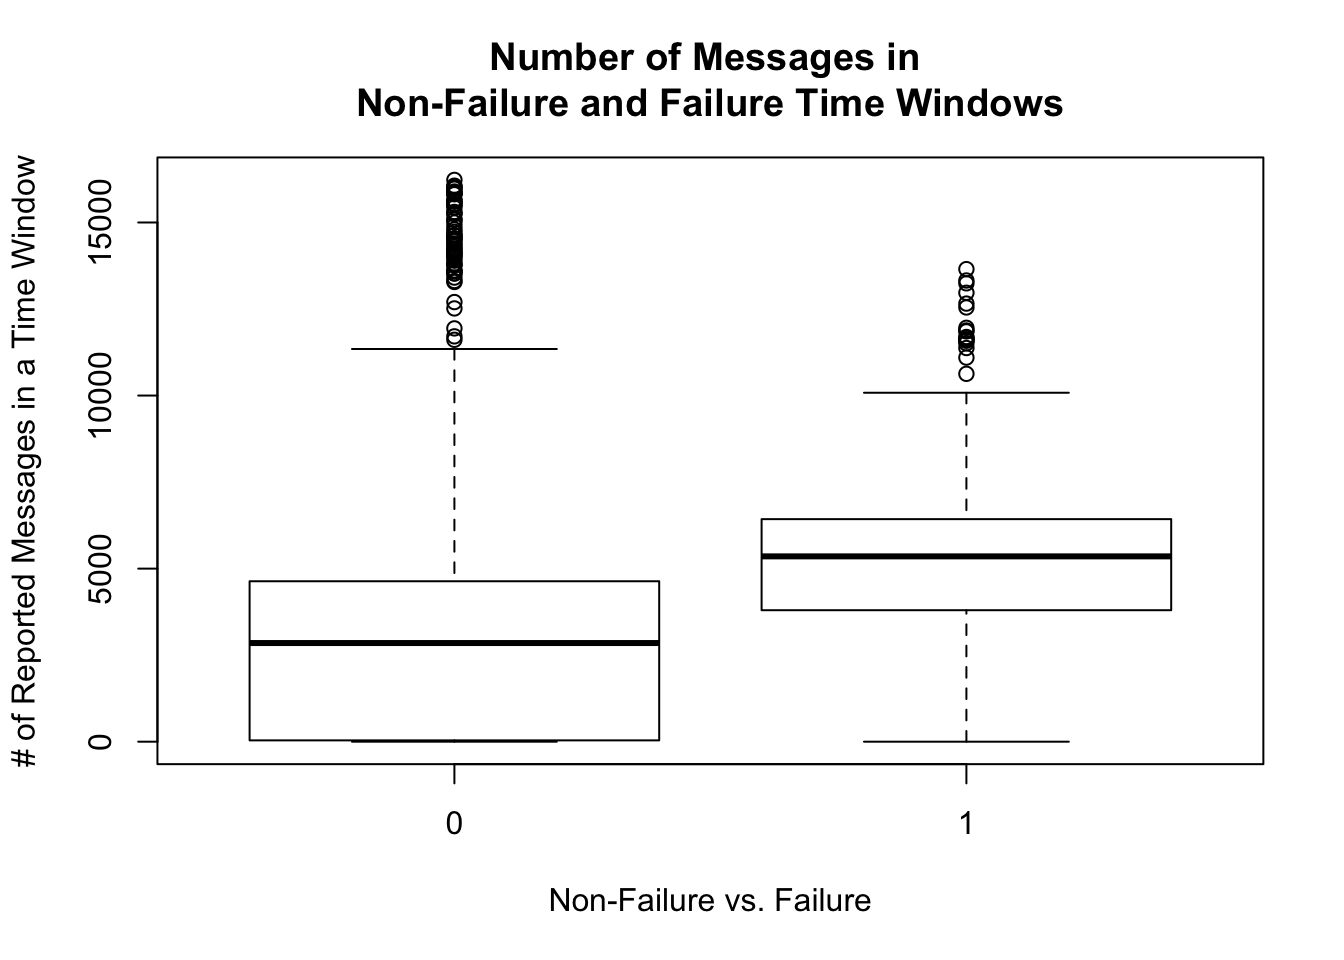
\includegraphics[width=#1]{MemLeakCompare}
  \caption[\ac{SVM} Memory Leak Performance Comparison]{Number of observations
  in a given thirty second time window where `1' represents a window during
  which failure occurred and `0' represents a window during which no failure
  occurred.}
  \label{fig:memLeakCompare}
 \end{center}
\end{figure}
}

%%%%   SMV   %%%%
% Pre-Update
\newcommand{\figMemLeakPreUpdateSVMPerf}{\begin{figure*}
  \centering
  \subfigure[Precision/Recall Curve.]{
    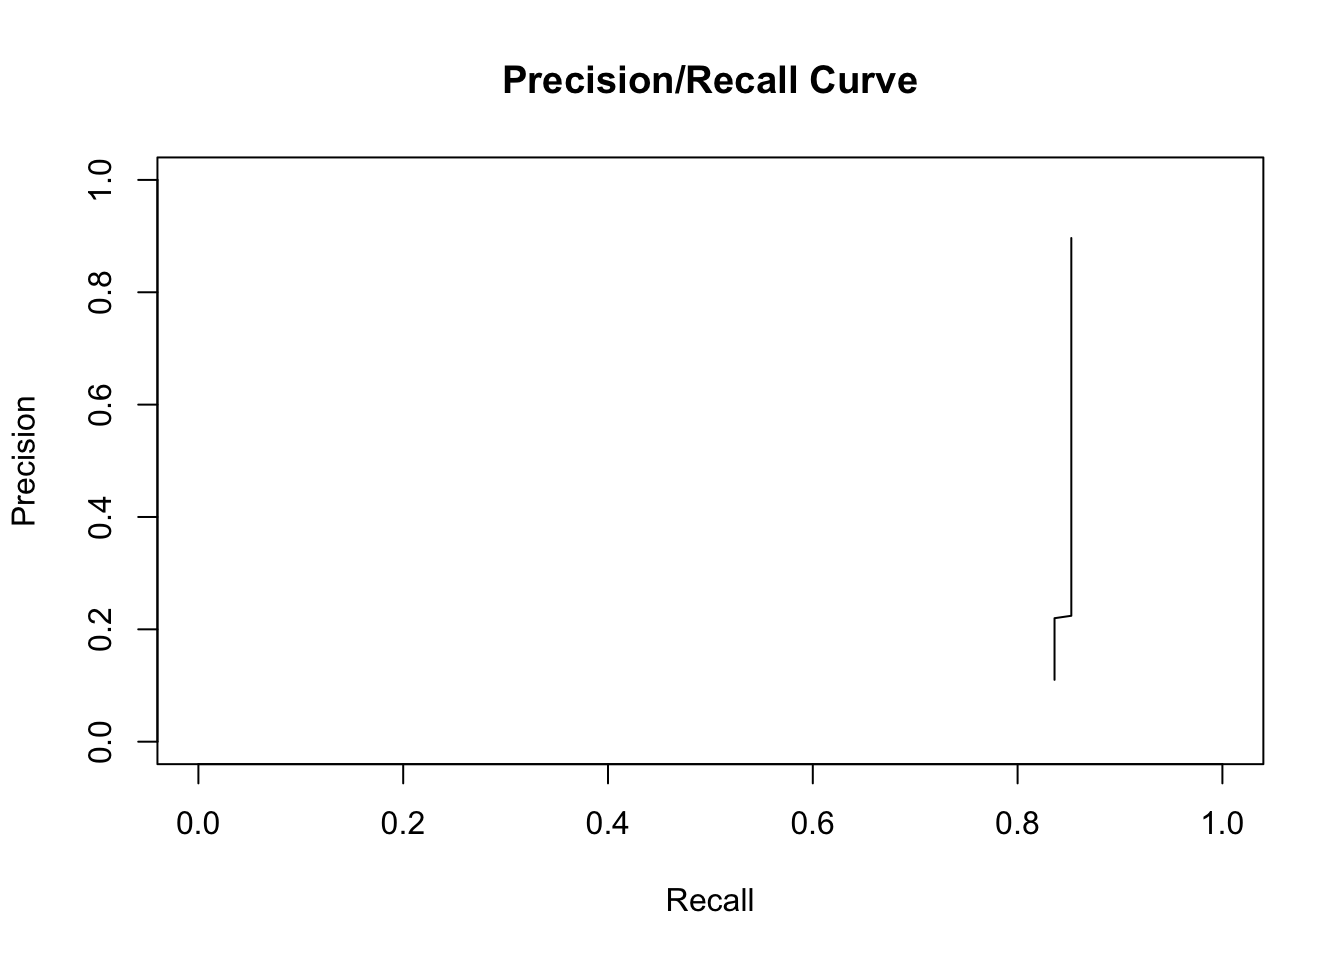
\includegraphics[width=0.45\textwidth]{results/pre-update/memleak/svm-prc}
  }
  \subfigure[\ac{ROC} Curve (\ac{AUC} = 0.8664).]{
    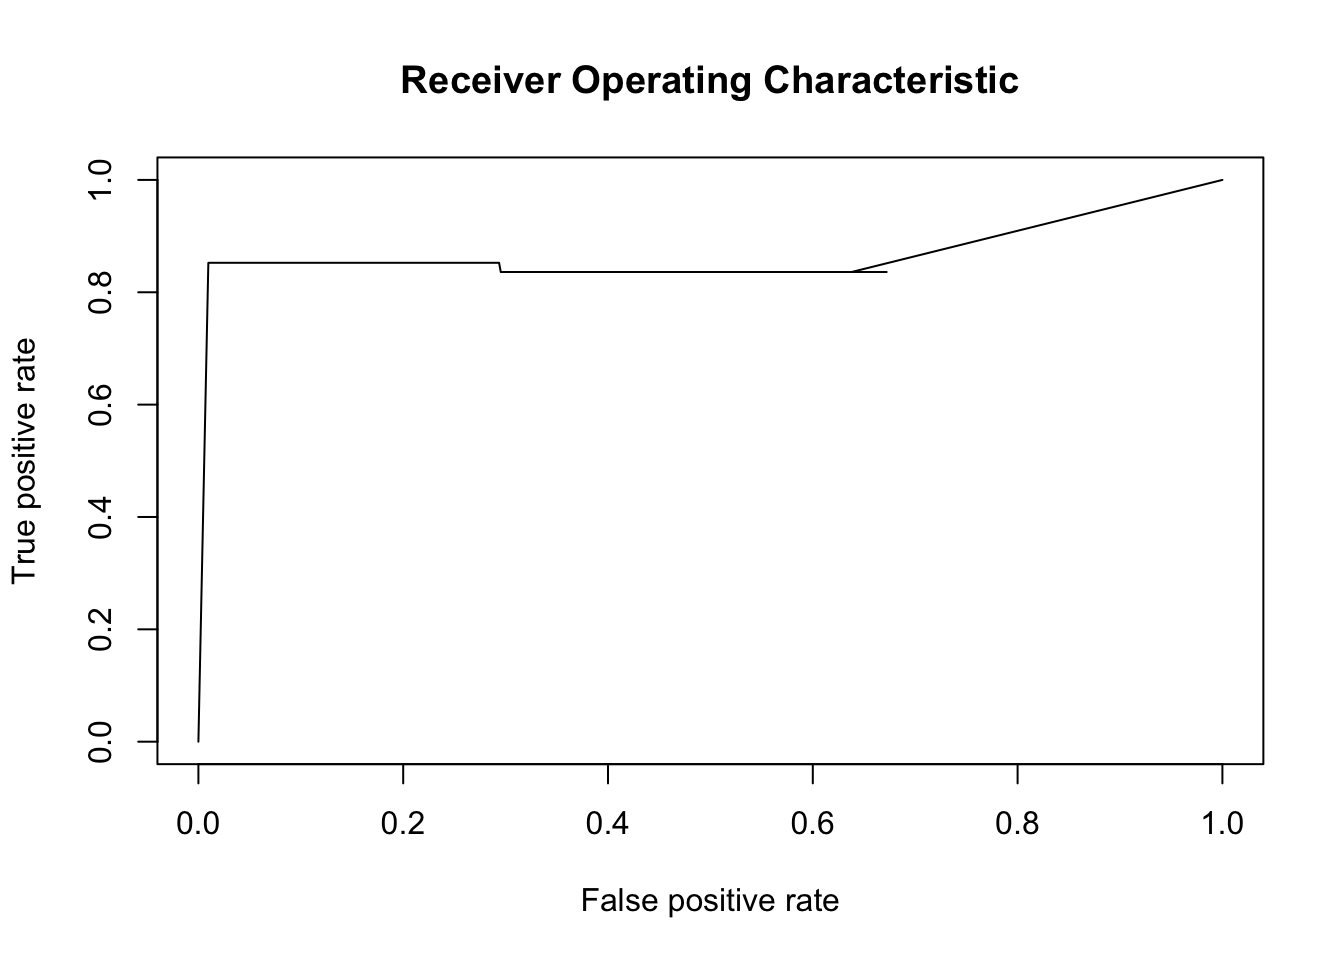
\includegraphics[width=0.45\textwidth]{results/pre-update/memleak/svm-roc}
  }
  \caption[Pre-Update, Memory Leak \ac{SVM} Performance]{Test data performance
  of the \ac{SVM} prediction method on failure data obtained by consuming all
  available memory until target application fails.}
  \label{fig:memLeakPreUpdateSVMPerf}
\end{figure*}
}

% Post-Update (old model)

% Post-Update New Model

%%%%   BOOSTING   %%%%
% Pre-Update
\newcommand{\figMemLeakPreUpdateBoostingPerf}{\begin{figure*}
  \centering
  \subfigure[Precision/Recall Curve.]{
    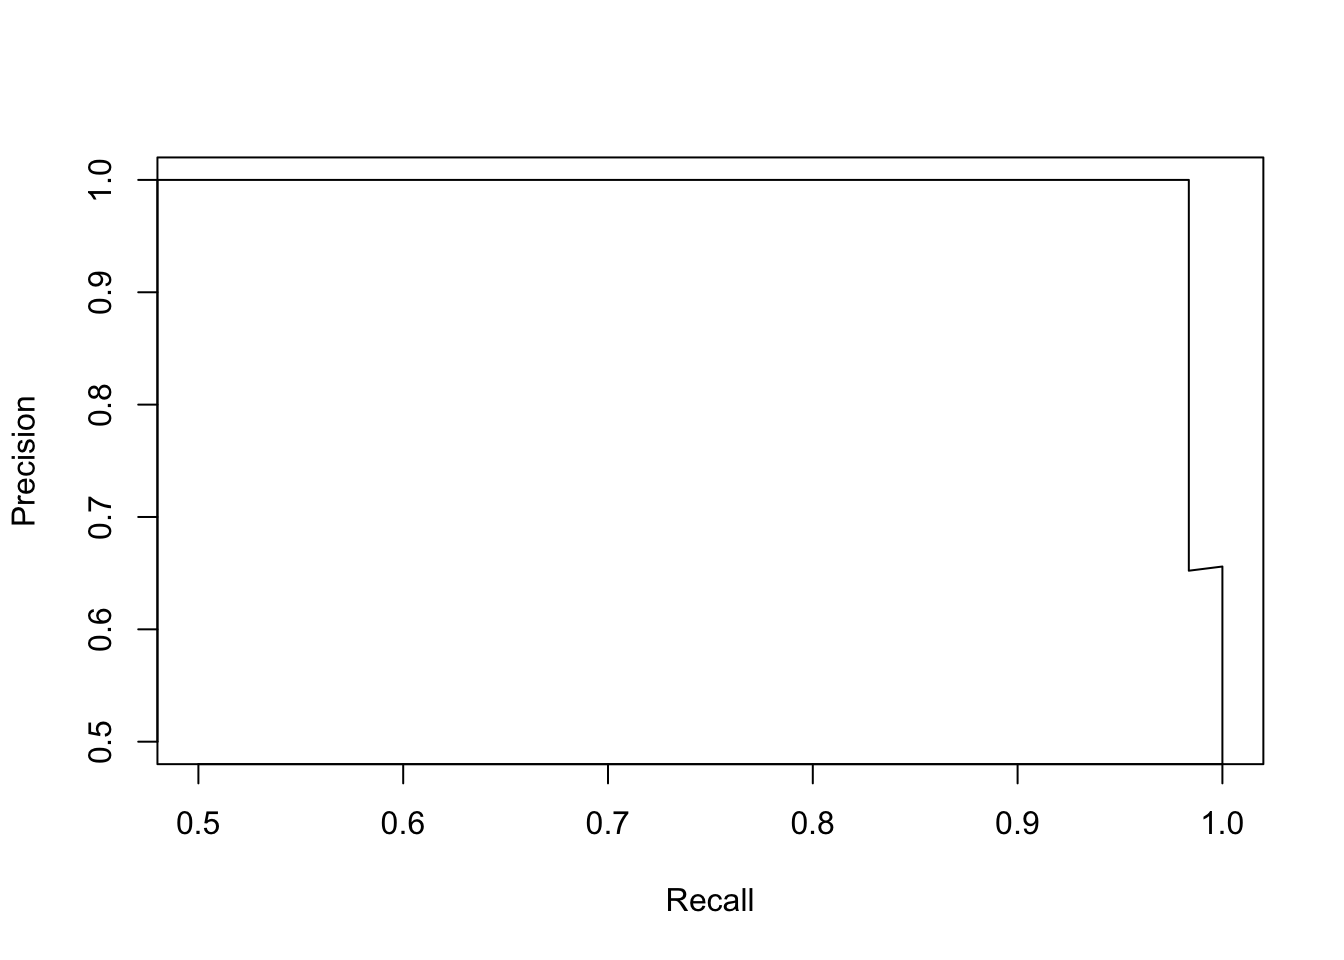
\includegraphics[width=0.45\textwidth]{results/pre-update/memleak/boosting-prc}
  }
  \subfigure[\ac{ROC} Curve (\ac{AUC} = 0.9984).]{
    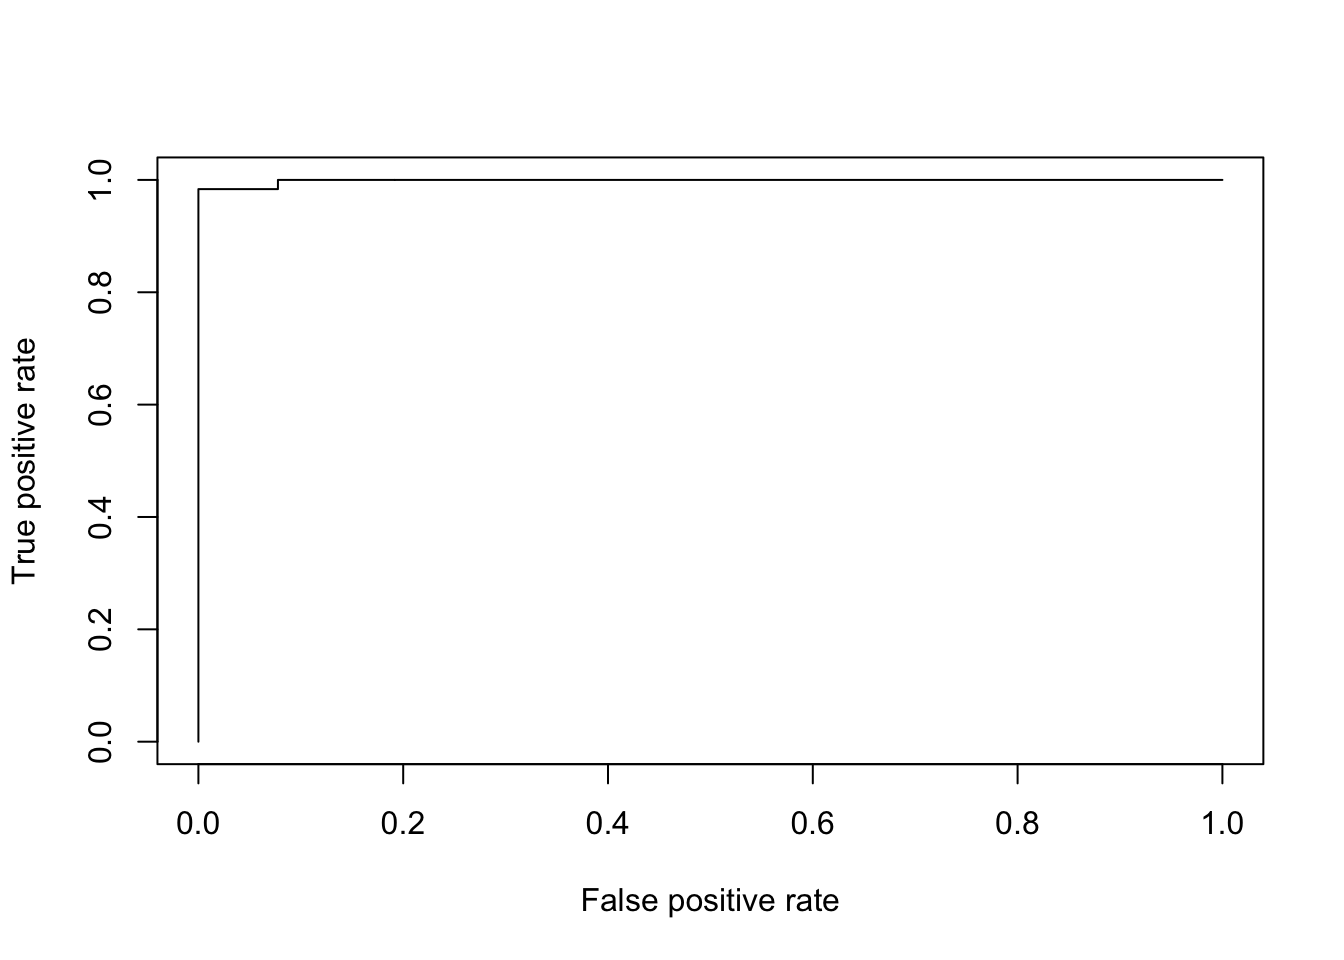
\includegraphics[width=0.45\textwidth]{results/pre-update/memleak/boosting-roc}
  }
  \caption[Pre-Update, Memory Leak Boosting Performance]{Test data performance
  of the boosting prediction method on failure data obtained by consuming all
  available memory until target application fails.}
  \label{fig:memLeakPreUpdateBoostingPerf}
\end{figure*}
}

% Post-Update (old model)
\newcommand{\figMemLeakPostUpdateSameBoostedModel}{\begin{figure*}
  \centering
  \subfigure[Precision/Recall Curve.]{
    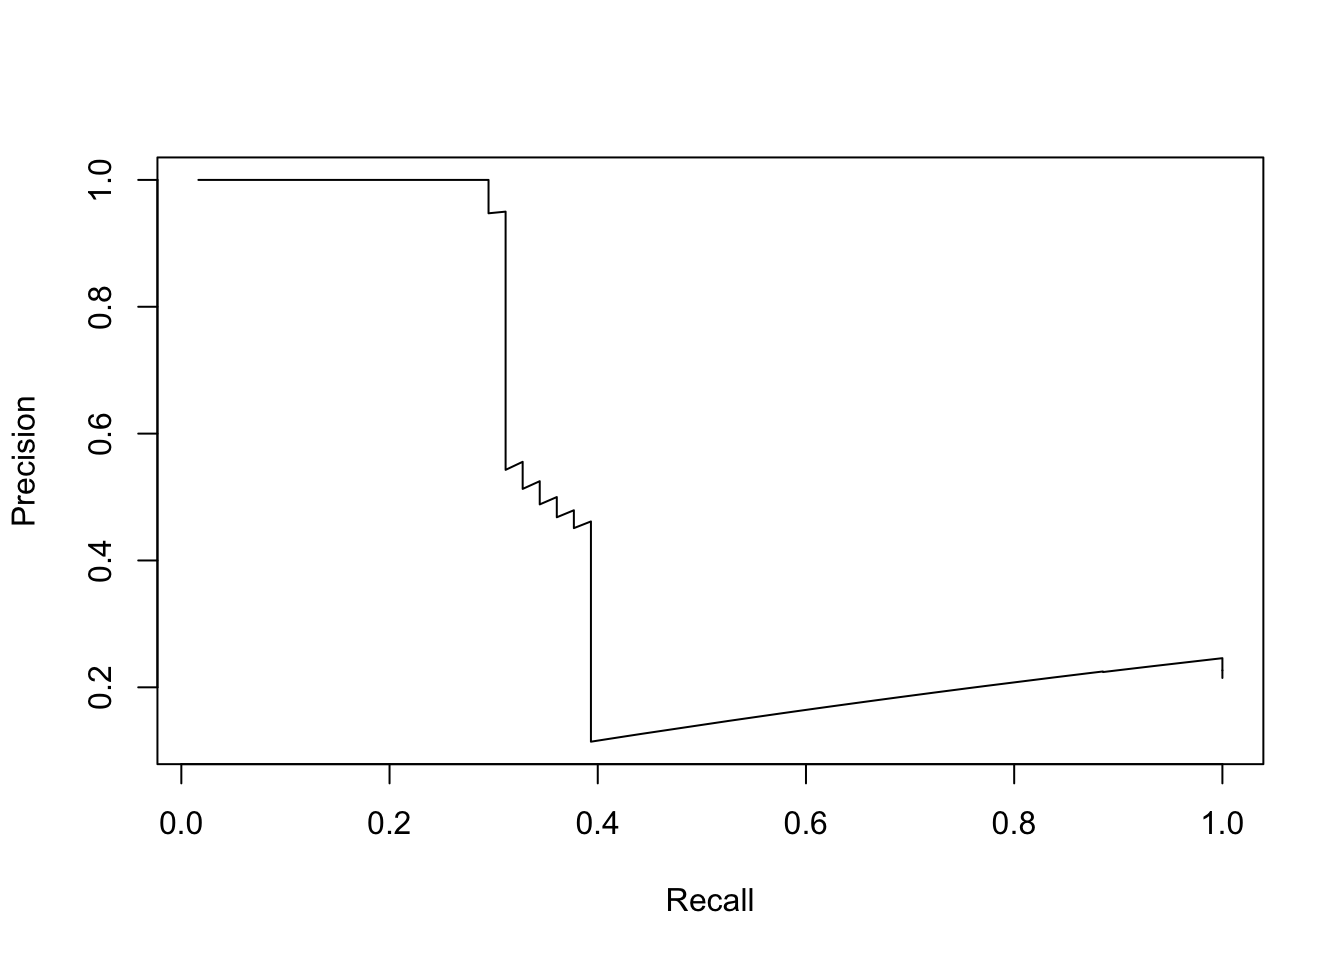
\includegraphics[width=0.45\textwidth]{results/post-update/memleak/boost-samemodel-prc}
  }
  \subfigure[\ac{ROC} Curve (\ac{AUC} = 0.4854).]{
    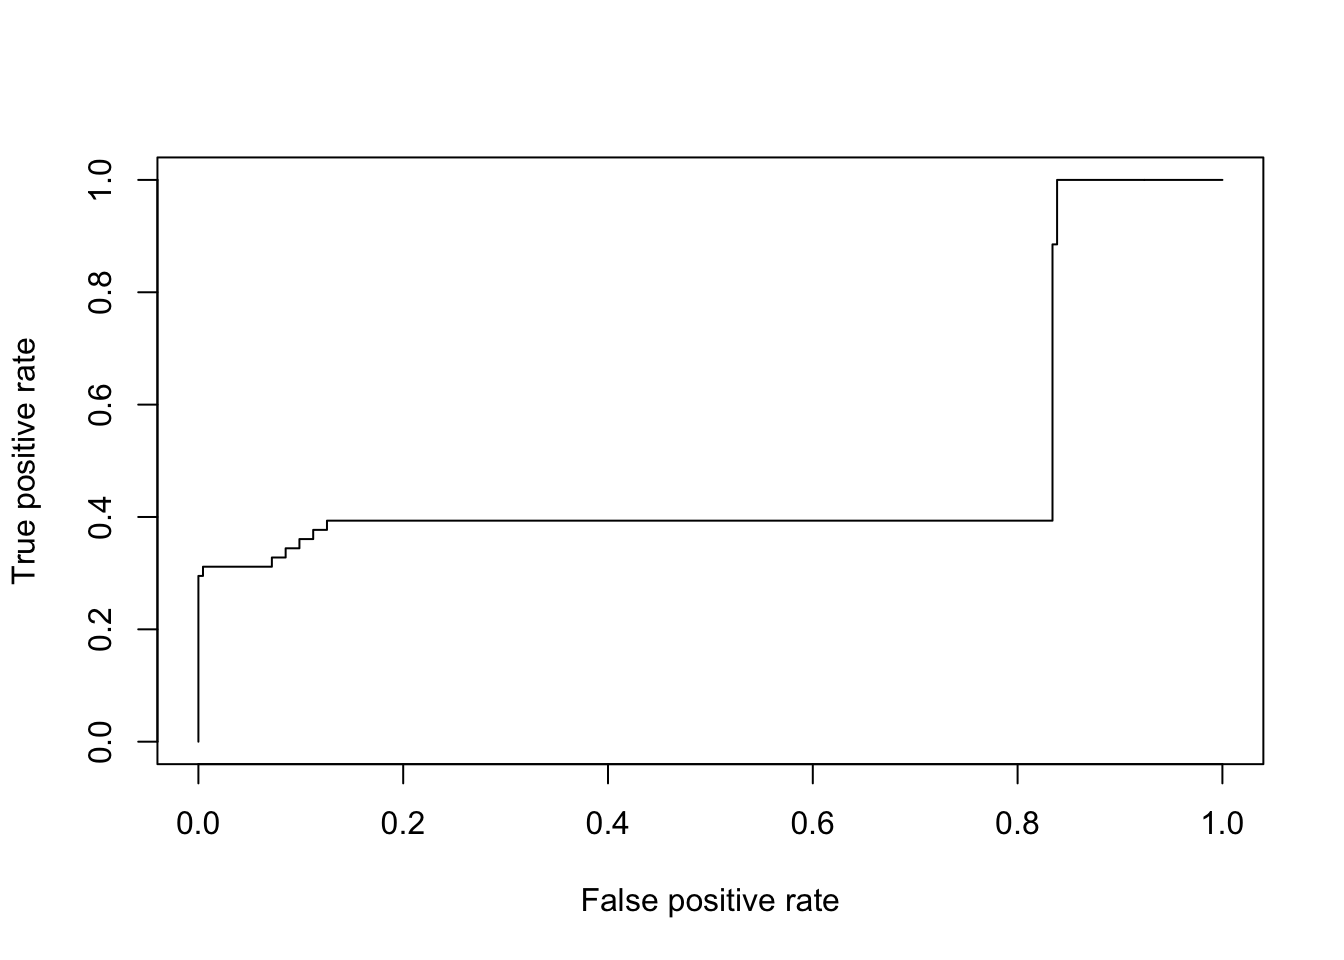
\includegraphics[width=0.45\textwidth]{results/post-update/memleak/boost-samemodel-roc}
  }
  \caption[Post-Update, Memory Leak Using Old Model Performance]{Performance of
  the boosting prediction method trained on failure data created before the
  software update obtained by consuming all available memory until target
  application fails.}
  \label{fig:memLeakPostUpdateSameBoostedModel}
\end{figure*}
}

% Post-Update New Model
\newcommand{\figMemLeakPostUpdateBoostingPerf}{\begin{figure*}
  \centering
  \subfigure[Precision/Recall Curve.]{
    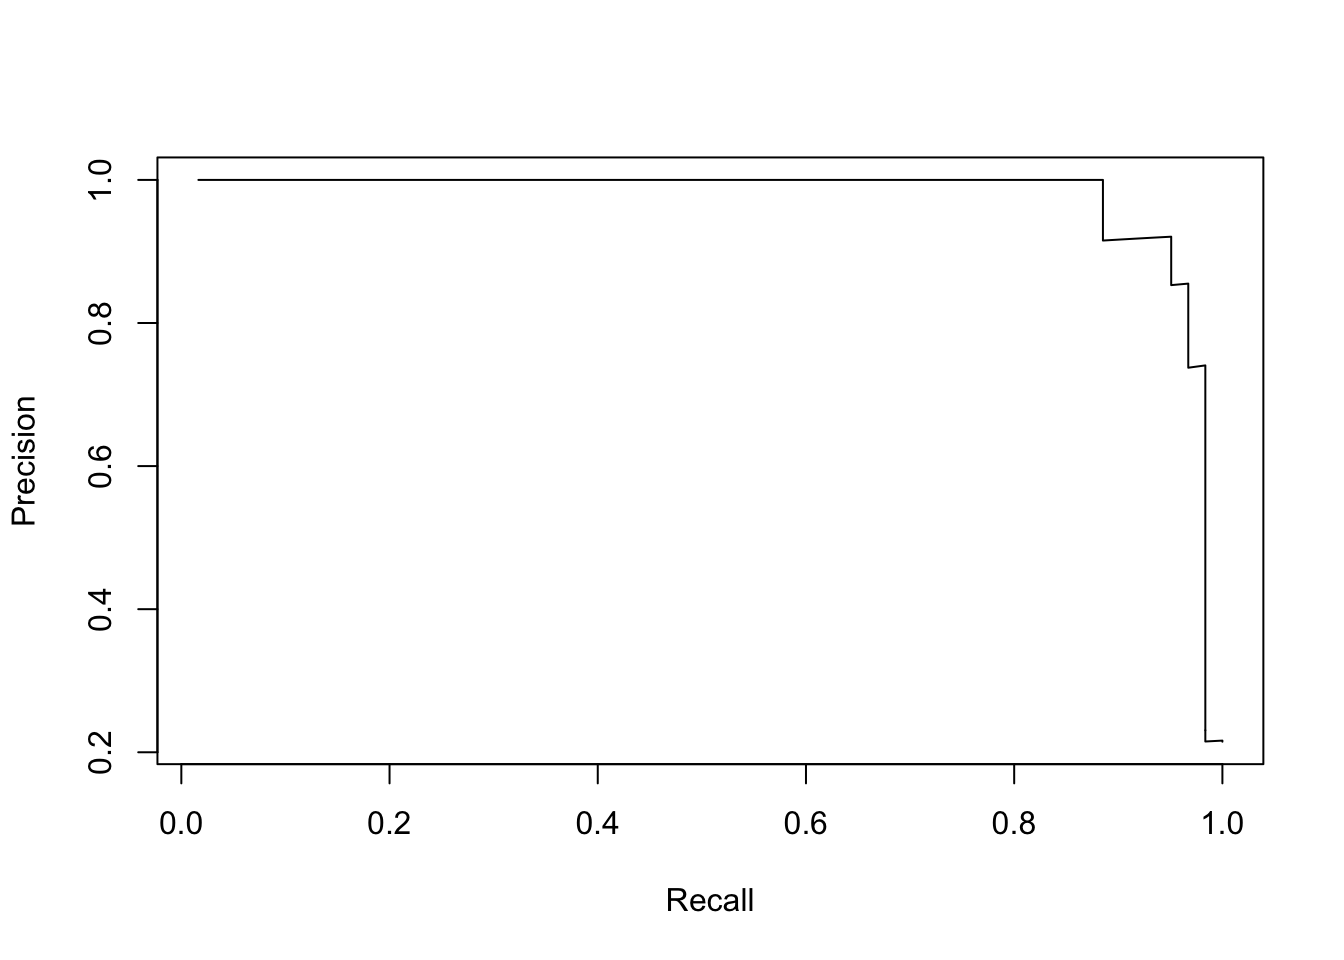
\includegraphics[width=0.45\textwidth]{results/post-update/memleak/boost-prc}
  }
  \subfigure[\ac{ROC} Curve (\ac{AUC} = 0.9801).]{
    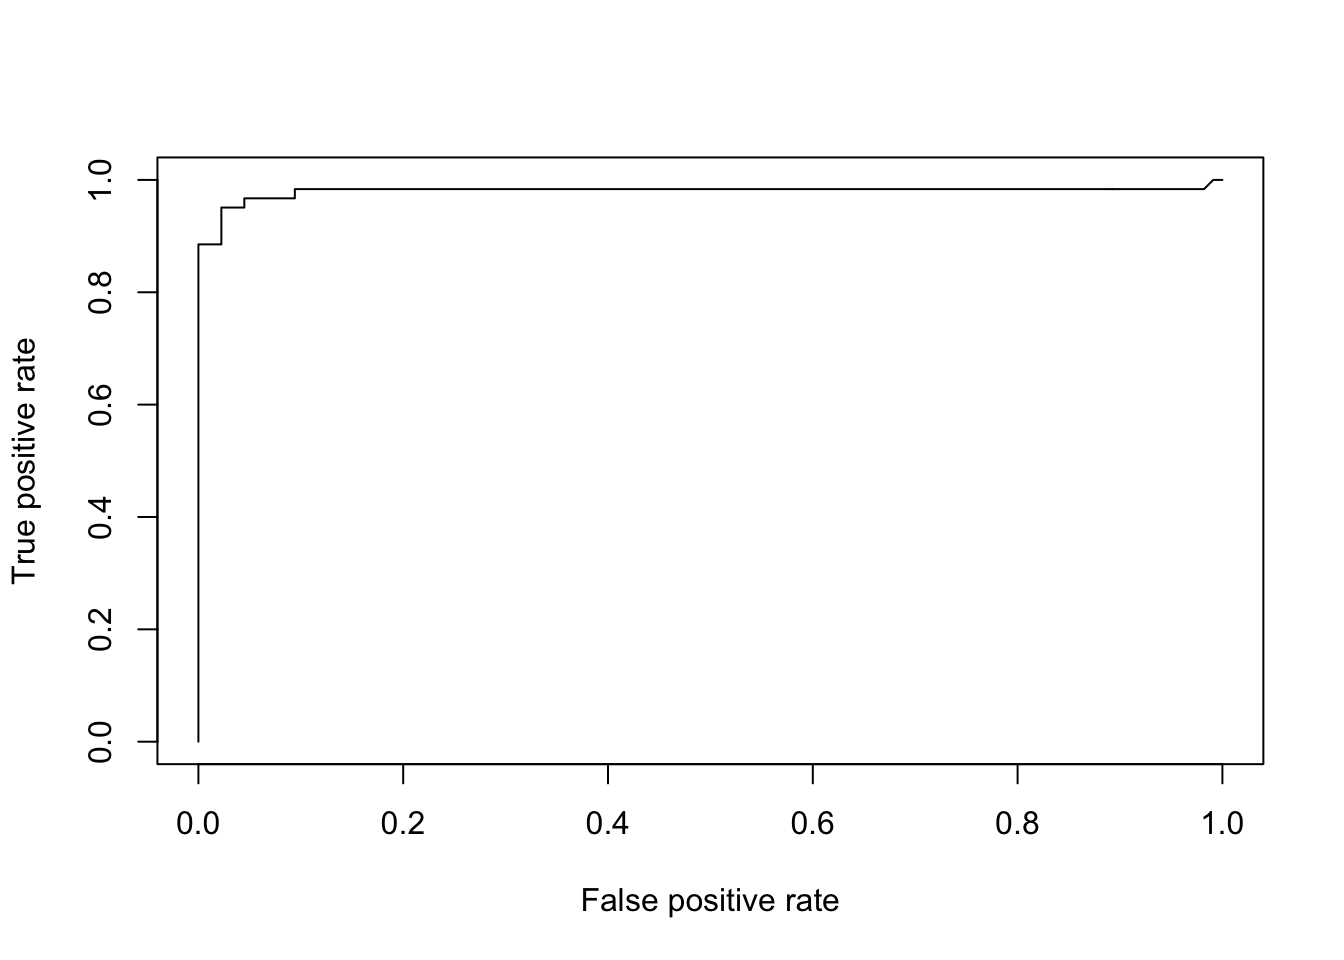
\includegraphics[width=0.45\textwidth]{results/post-update/memleak/boost-roc}
  }
  \caption[Post-Update, Memory Leak Using New Model Performance]{Performance of
  the boosting prediction method trained on failure data created after the
  software update obtained by consuming all available memory until target
  application fails.}
  \label{fig:memLeakPostUpdateBoostingPerf}
\end{figure*}
}

\newcommand{\figDPLGConceptDiagram}[1]{\begin{figure}
  \centering 
  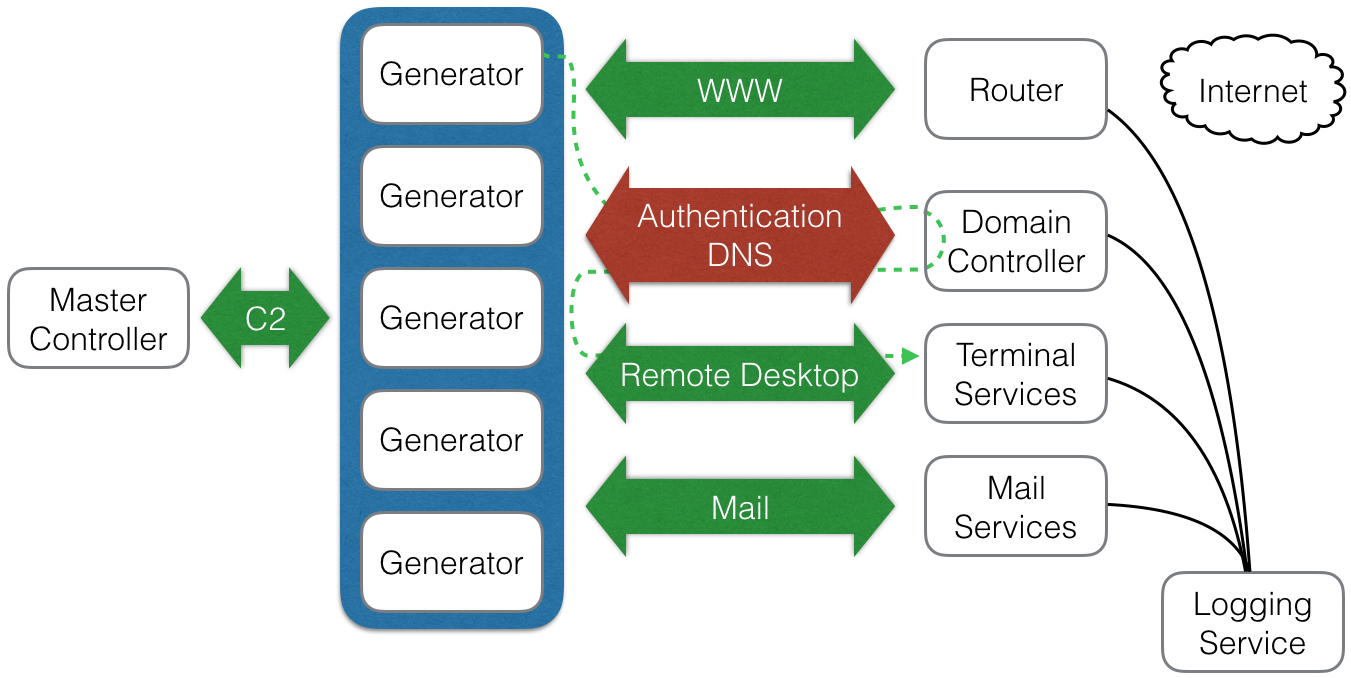
\includegraphics[width=#1]{DPLG/dplgConceptDiagram}
  \caption[Concept Diagram]{How each type of traffic that is generated is
  routed.  Log events are offloaded to logging service for further analysis.}
  \label{fig:conceptDiagram} 
  \end{figure}
}

\newcommand{\figDPLGAllModsClientMetrics}[1]{\begin{figure}
  \centering
  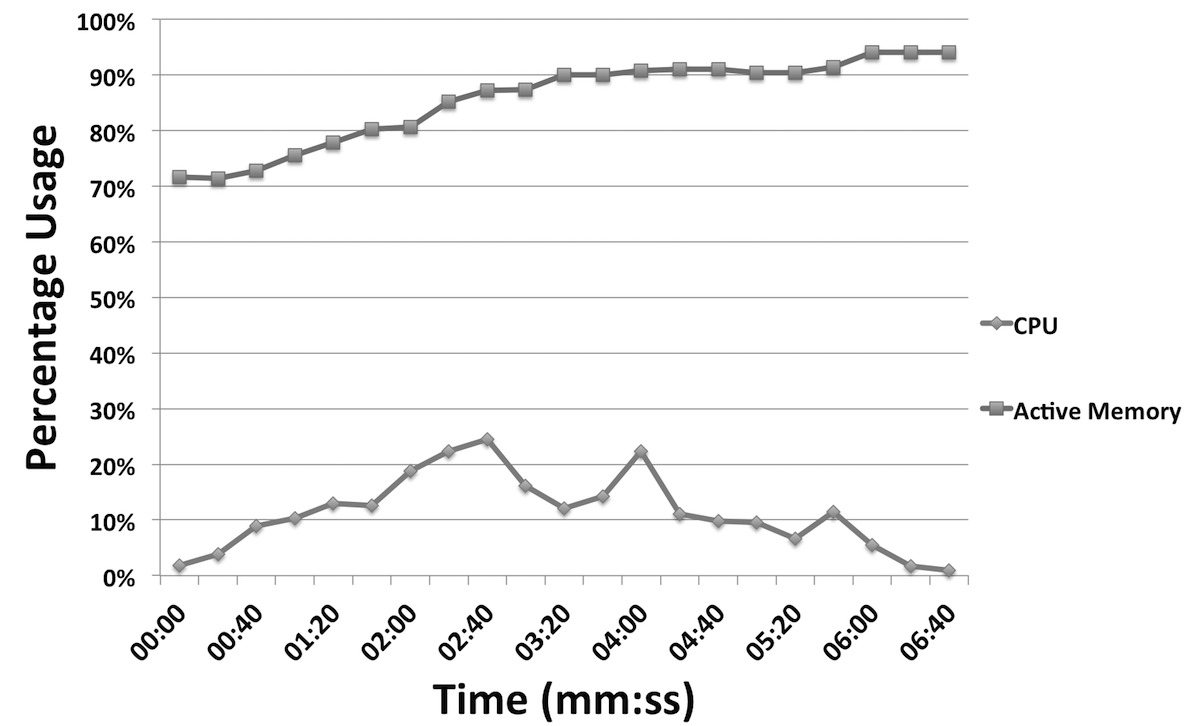
\includegraphics[width=#1]{DPLG/allModsClientMetrics}
  \caption[Test 2:  Client Metrics]{Client CPU and memory utilization during
  the second test.} \label{fig:allModsClientMetrics}
  \end{figure}
}


\newcommand{\tabFaults}{
\begin{table}[htbp]
  \centering
  \caption{Table of Faults Injected~\cite{gswfit}.}\label{tab:faults}
\begin{tabular}{ | c | l | c | } 
\hline
	\textbf{Type}  & \textbf{Description}  & \textbf{ODC Classes}  \\ \hline \hline
	MIFS  & Missing "If (cond) \{ statement(s) \}"  & Algorithm  \\ \hline
	MFC  & Missing function call  & Algorithm  \\ \hline
	MLAC  & Missing "AND EXPR" in expression used as branch & Checking  \\ \hline
	MLPC  & Missing small and localized part of the algorithm  & Algorithm  \\ \hline
	WVAV  & Wrong value assigned to a value  & Assignment  \\ \hline
	MVI  & Missing variable initialization  & Assignment  \\ \hline
	MVAV  & Missing variable assignment using a value  & Assignment  \\ \hline
	WPFV  & Wrong variable used in parameter of function call  & Interface  \\ \hline
\end{tabular}
\end{table}
}

\newcommand{\tabTranslationThirtyTwo}{
\begin{table}[htbp]
  \centering
  \caption{Funtion Entry/Exit Patterns
  (IA32)~\cite{gswfit}.}\label{tab:translationThirtyTwo}
\begin{tabular}{ | l | l | l | l | }
\hline
	\multicolumn{2}{|c|}{\textbf{Module Entry Point}}& 
  \multicolumn{2}{c|}{\textbf{Module Exit Point}} \\ \hline

	\textbf{Instruction Sequence} & \textbf{Explanation} &
  \textbf{Instruction Sequence} & \textbf{Explanation} \\ \hline \hline

	push ebp & stack frame & move esp,ebp & stack frame \\ \hline
	mov ebp, esp & setup & pop ebp & cleanup \\ \hline
	sub esp, \emph{immed} &  & ret &  \\ \hline
\end{tabular}
\end{table}
}

\newcommand{\tabTranslationSixtyFour}{
\begin{table}[htbp]
  \centering
  \caption{Funtion Entry/Exit Patterns
  (x86-64)~\cite{gswfit}.}\label{tab:translationSixtyFour}
\begin{tabular}{ | l | l | l | l | }
\hline
	\multicolumn{2}{|c|}{\textbf{Module Entry Point}}& 
  \multicolumn{2}{c|}{\textbf{Module Exit Point}} \\ \hline

	\textbf{Instruction Sequence} & \textbf{Explanation} & 
  \textbf{Instruction Sequence} & \textbf{Explanation} \\ \hline \hline

	push rbp & stack frame & add rsp, \emph{immed} & stack frame \\ \hline
	sub rsp, \emph{immed} &  & pop rbp & cleanup \\ \hline
	mov rbp, rdx & setup & ret &  \\ \hline
\end{tabular}
\end{table}
}

\newcommand{\tabHypervisorOne}{
\begin{table}[htbp]
  \centering
  \caption{Hypervisor 1 Configuration (Sandbox/Target).} \label{tab:hyp1}
  \begin{tabular}{ | c | l | l | c | l |}
    \hline
    Qty. & Role   & Operating System    & CPU / Mem. \\ \hline\hline
    1    & DC     & Win. Server 2008 R2 & 2 / 2 GB   \\ \hline
    5    & Client & Win. 7              & 1 / 512 MB \\ 
    \hline
  \end{tabular}
\end{table}
}


\newcommand{\tabHypervisorTwo}{
\begin{table}[htbp]
  \centering
  \caption{Hypervisor 2 Configuration (Controller).} \label{tab:hyp2}
  \begin{tabular}{ | c | l | l | c | l |}
    \hline
    Qty. & Role & Operating System    & CPU / Mem. \\ \hline\hline
    1    & RDP  & Win. Server 2008 R2 & 1 / 4 GB   \\ \hline
    1    & Log  & Ubuntu 14.04 LTS    & 1 / 1 GB   \\ 
    \hline
  \end{tabular}
\end{table}
}

\newcommand{\tabMessage}{
\begin{table}[!ht] \centering
  \caption{Typical authentication message sent as keys that correspond to the
  values as designated in the \emph{Snare} protocol for MSWinEventLog used by
  the SolarWinds syslog agent.} \label{tab:message}
  \begin{tabular}{ | l | l | }
    \hline
      Key                 & Value                               \\ \hline\hline
      HostName            & dc.afnet.com                        \\ \hline
      Criticality         & 5                                   \\ \hline
      EventLogSource      & Security                            \\ \hline
      Counter             & 3                                   \\ \hline
      SubmitTime          & Sun May 08 14:31:50 2016            \\ \hline
      EventID             & 4672                                \\ \hline
      SourceName          & Microsoft-Windows-Security-Auditing \\ \hline
      UserName            & N/A                                 \\ \hline
      SIDType             & Audit Success                       \\ \hline
      EventLogType        & dc.afnet.com                        \\ \hline
      ComputerName        & 12548                               \\ \hline
      CategoryString      & Special privileges assigned to\dots \\ \hline
      ExtendedDataString  & Security ID:  S-1-5-21-2379403\dots \\ 
    \hline
  \end{tabular}
\end{table}
}

\newcommand{\tabSlidingWindow}{
\begin{table}[!ht] \centering
  \caption{Sample time window after message translation.} \label{tab:window}
  \begin{tabular}{ | l | l | }
    \hline
      Key                         & Value \\ \hline\hline
      FailureWindow               & 0     \\ \hline
      NumObservations             & 2     \\ \hline
      Criticality: 6              & 2     \\ \hline
      Criticality: 2              & 0     \\ \hline
      Criticality: 4              & 0     \\ \hline
      EventLogSource: Application & 1     \\ \hline
      EventLogSource: System      & 1     \\ 
    \hline
  \end{tabular}
\end{table}
}

\newcommand{\tabMemLeakPreUpdateSVMStats}{
\begin{table}[!t] \centering
  \caption[Pre-Update, Memory Leak, SVM Statistics]{Classification statistics
  on test data created before software updates.}
  \label{tab:memLeakPreUpdateSVMStats}
  \begin{tabular}{ | l | l | }
    \hline
      Statistic           & Value  \\ \hline\hline
      True Positive Rate  & 0.8525 \\ \hline
      False Positive Rate & 0.0098 \\ \hline
      Accuracy            & 0.9777 \\ \hline
      Precision           & 0.8966 \\ \hline
      Recall              & 0.8525 \\ \hline
      F-Measure           & 0.8739 \\
    \hline
  \end{tabular}
\end{table}
}
%%%%%%%%%%%%%%%%%%%%%%%%%%%%%%%%%%%%%%%%%%%%%%%%%%%%%%%%%%%%%%%%%%%%%%%%%%%%%%%
%%%%   SVM   %%%%
% Pre-Update
\newcommand{\tabMemLeakPreUpdateSVMConfusionMatrix}{
  \begin{table}[!ht]
    \centering
    \caption[Pre-Update, Memory Leak, SVM Confusion Matrix]{Confusion matrix on
    test data created before software updates on threshold with highest
    F-Measure (0.8739) using SVM.}
    \label{tab:memLeakPreUpdateSVMConfusionMatrix}
    \begin{tabular}{llll}
                                                               &                                       & \multicolumn{2}{c}{\textbf{Actual}}                                        \\ \cline{3-4} 
                                                               & \multicolumn{1}{l|}{}                 & \multicolumn{1}{l|}{\textbf{Fail}} & \multicolumn{1}{l|}{\textbf{No-Fail}} \\ \cline{2-4} 
      \multicolumn{1}{c|}{\multirow{2}{*}{\textbf{Predicted}}} & \multicolumn{1}{l|}{\textbf{Fail}}    & \multicolumn{1}{l|}{52}            & \multicolumn{1}{l|}{6}                \\ \cline{2-4} 
      \multicolumn{1}{c|}{}                                    & \multicolumn{1}{l|}{\textbf{No-Fail}} & \multicolumn{1}{l|}{9}             & \multicolumn{1}{l|}{607}              \\ \cline{2-4} 
    \end{tabular}
  \end{table}
}

% Post-Update (old model)

% Post-Update New Model

%%%%   BOOSTING   %%%%
% Pre-Update
\newcommand{\tabMemLeakPreUpdateBoostingConfusionMatrix}{
  \begin{table}[!ht]
    \centering
    \caption[Pre-Update, Memory Leak, Boosting Confusion Matrix]{Confusion
    matrix on test data created before software updates on threshold with
    highest F-Measure (0.9917) using boosting.}
    \label{tab:memLeakPreUpdateBoostingConfusionMatrix}
    \begin{tabular}{llll}
                                                               &                                       & \multicolumn{2}{c}{\textbf{Actual}}                                        \\ \cline{3-4} 
                                                               & \multicolumn{1}{l|}{}                 & \multicolumn{1}{l|}{\textbf{Fail}} & \multicolumn{1}{l|}{\textbf{No-Fail}} \\ \cline{2-4} 
      \multicolumn{1}{c|}{\multirow{2}{*}{\textbf{Predicted}}} & \multicolumn{1}{l|}{\textbf{Fail}}    & \multicolumn{1}{l|}{60}            & \multicolumn{1}{l|}{0}                \\ \cline{2-4} 
      \multicolumn{1}{c|}{}                                    & \multicolumn{1}{l|}{\textbf{No-Fail}} & \multicolumn{1}{l|}{1}             & \multicolumn{1}{l|}{412}              \\ \cline{2-4} 
    \end{tabular}
  \end{table}
}

% Post-Update (old model)
\newcommand{\tabMemLeakPostUpdateBoostingSameModelConfusionMatrix}{
  \begin{table}[!ht]
    \centering
    \caption[Post-Update, Memory Leak, Same Model, Confusion
    Matrix]{Post-update failure data confusion matrix on threshold with highest
    F-Measure (0.4691) using model trained on failure data generated before
    software update.}
    \label{tab:memLeakPostUpdateBoostingSameModelConfusionMatrix}
    \begin{tabular}{llll}
                                                               &                                       & \multicolumn{2}{c}{\textbf{Actual}}                                        \\ \cline{3-4} 
                                                               & \multicolumn{1}{l|}{}                 & \multicolumn{1}{l|}{\textbf{Fail}} & \multicolumn{1}{l|}{\textbf{No-Fail}} \\ \cline{2-4} 
      \multicolumn{1}{c|}{\multirow{2}{*}{\textbf{Predicted}}} & \multicolumn{1}{l|}{\textbf{Fail}}    & \multicolumn{1}{l|}{19}            & \multicolumn{1}{l|}{1}                \\ \cline{2-4} 
      \multicolumn{1}{c|}{}                                    & \multicolumn{1}{l|}{\textbf{No-Fail}} & \multicolumn{1}{l|}{42}            & \multicolumn{1}{l|}{222}              \\ \cline{2-4} 
    \end{tabular}
  \end{table}
}

% Post-Update New Model
\newcommand{\tabMemLeakPostUpdateBoostingConfusionMatrix}{
  \begin{table}[!ht]
    \centering
    \caption[Post-Update, Memory Leak, New Model, Confusion
    Matrix]{Post-update failure data confusion matrix on threshold with highest
    F-Measure (0.9355) using model trained on failure data generated after
    software update.}
    \label{tab:memLeakPostUpdateBoostingConfusionMatrix}
    \begin{tabular}{llll}
                                                               &                                       & \multicolumn{2}{c}{\textbf{Actual}}                                        \\ \cline{3-4} 
                                                               & \multicolumn{1}{l|}{}                 & \multicolumn{1}{l|}{\textbf{Fail}} & \multicolumn{1}{l|}{\textbf{No-Fail}} \\ \cline{2-4} 
      \multicolumn{1}{c|}{\multirow{2}{*}{\textbf{Predicted}}} & \multicolumn{1}{l|}{\textbf{Fail}}    & \multicolumn{1}{l|}{58}            & \multicolumn{1}{l|}{5}                \\ \cline{2-4} 
      \multicolumn{1}{c|}{}                                    & \multicolumn{1}{l|}{\textbf{No-Fail}} & \multicolumn{1}{l|}{3}             & \multicolumn{1}{l|}{218}              \\ \cline{2-4} 
    \end{tabular}
  \end{table}
}

%%%%%%%%%%%%%%%%%%%%%%%%%%%%%%%%%%%%%%%%%%%%%%%%%%%%%%%%%%%%%%%%%%%%%%%%%%%%%%%
\newcommand{\tabModelSelection}{
\begin{table*}[!t]
  \centering
  \caption{Cross-validation runs on training data for model selection and
  resulting classification accuracy.}
  \label{tab:model:selection}
  \begin{tabular}{cllllllllllll}
    \multicolumn{1}{l}{}                       & \multicolumn{12}{c}{{\ul \textbf{Amount of Training Data}}}                                                                                                                                                                                         \\ \cline{2-13} 
    \multicolumn{1}{l|}{{\ul \textbf{Window}}} & \multicolumn{4}{c}{One Failure}                                             & \multicolumn{4}{c}{Two Failures}                                                & \multicolumn{4}{c|}{Four Failures}                                              \\ \cline{2-13} 
    \multicolumn{1}{c|}{\multirow{2}{*}{30s}}  & \textbf{Linear:}  & 0.0557 & \textbf{Poly:}   & \multicolumn{1}{l|}{0.0523} & \textbf{Linear:}  & 0.0756 & \textbf{Poly:}   & \multicolumn{1}{l|}{0.0659} & \textbf{Linear:}  & 0.0733 & \textbf{Poly:}   & \multicolumn{1}{l|}{0.0547} \\
    \multicolumn{1}{c|}{}                      & \textbf{Sigmoid:} & 0.0626 & \textbf{Radial:} & \multicolumn{1}{l|}{0.0459} & \textbf{Sigmoid:} & 0.0591 & \textbf{Radial:} & \multicolumn{1}{l|}{0.0438} & \textbf{Sigmoid:} & 0.0794 & \textbf{Radial:} & \multicolumn{1}{l|}{0.0542} \\ \cline{2-13} 
    \multicolumn{1}{c|}{\multirow{2}{*}{60s}}  & \textbf{Linear:}  & 0.0628 & \textbf{Poly:}   & \multicolumn{1}{l|}{0.0662} & \textbf{Linear:}  & 0.0779 & \textbf{Poly:}   & \multicolumn{1}{l|}{0.064}  & \textbf{Linear:}  & 0.0791 & \textbf{Poly:}   & \multicolumn{1}{l|}{0.0779} \\
    \multicolumn{1}{c|}{}                      & \textbf{Sigmoid:} & 0.1084 & \textbf{Radial:} & \multicolumn{1}{l|}{0.0487} & \textbf{Sigmoid:} & 0.1328 & \textbf{Radial:} & \multicolumn{1}{l|}{0.071}  & \textbf{Sigmoid:} & 0.2159 & \textbf{Radial:} & \multicolumn{1}{l|}{0.0797} \\ \cline{2-13} 
    \multicolumn{1}{c|}{\multirow{2}{*}{90s}}  & \textbf{Linear:}  & 0.1272 & \textbf{Poly:}   & \multicolumn{1}{l|}{0.0897} & \textbf{Linear:}  & 0.1131 & \textbf{Poly:}   & \multicolumn{1}{l|}{0.0732} & \textbf{Linear:}  & 0.0826 & \textbf{Poly:}   & \multicolumn{1}{l|}{0.0543} \\
    \multicolumn{1}{c|}{}                      & \textbf{Sigmoid:} & 0.1792 & \textbf{Radial:} & \multicolumn{1}{l|}{0.0779} & \textbf{Sigmoid:} & 0.2684 & \textbf{Radial:} & \multicolumn{1}{l|}{0.0757} & \textbf{Sigmoid:} & 0.2404 & \textbf{Radial:} & \multicolumn{1}{l|}{0.0552} \\ \cline{2-13} 
    \multicolumn{1}{c|}{\multirow{2}{*}{120s}} & \textbf{Linear:}  & 0.132  & \textbf{Poly:}   & \multicolumn{1}{l|}{0.104}  & \textbf{Linear:}  & 0.1452 & \textbf{Poly:}   & \multicolumn{1}{l|}{0.0785} & \textbf{Linear:}  & 0.0998 & \textbf{Poly:}   & \multicolumn{1}{l|}{0.0705} \\
    \multicolumn{1}{c|}{}                      & \textbf{Sigmoid:} & 0.204  & \textbf{Radial:} & \multicolumn{1}{l|}{0.104}  & \textbf{Sigmoid:} & 0.2864 & \textbf{Radial:} & \multicolumn{1}{l|}{0.0585} & \textbf{Sigmoid:} & 0.3056 & \textbf{Radial:} & \multicolumn{1}{l|}{0.0792} \\ \cline{2-13} 
  \end{tabular}
\end{table*}
}

\makeglossaries
\newacronym{AFP}{AFP}{Adaptive Failure Prediction}
\newacronym{OFP}{OFP}{Online Failure Prediction}
\newacronym{CPU}{CPU}{Central Processing Unit}
\newacronym{G-SWFIT}{G-SWFIT}{Generic Software Fault Injection Technique}
\newacronym{W-SWFIT}{W-SWFIT}{Windows Software Fault Injection Tool}
\newacronym{CSCS}{CSCS}{Cyber Security and Control System}
\newacronym{NOS}{NOS}{Network Operation Squadrons}
\newacronym{DOD}{DOD}{Department of Defense}
\newacronym{GHSMM}{GHSMM}{Generalized Hidden Semi-Markov Model}
\newacronym{SVM}{SVM}{Support Vector Machine}
\newacronym{IP}{IP}{Internet Protocol}
\newacronym{CRISP-DM}{CRISP-DM}{Cross Industry Standard Process for Data Mining}
\newacronym{ROC}{ROC}{Receiver Operating Characteristic}
\newacronym{MS}{MS}{Microsoft}
\newacronym{AD}{AD}{Active Directory}
\newacronym{GB}{GB}{Gigabyte}
\newacronym{GHz}{GHz}{Gigahertz}
\newacronym{VM}{VM}{Virtual Machine}
\newacronym{PFM}{PFM}{Proactive Fault Management}
\newacronym{DC}{DC}{Domain Controller}
\newacronym{ASLR}{ASLR}{Address Space Layout Randomization}
\newacronym{DNS}{DNS}{Domain Name System}
\newacronym{D-PLG}{D-PLG}{Distributed PowerShell Load Generator}
\newacronym{RDP}{RDP}{Remote Desktop Protocol}
\newacronym{SQL}{SQL}{Structured Query Language}
\newacronym{API}{API}{Application Programming Interface}
\newacronym{TP}{TP}{True Positive}
\newacronym{FP}{FP}{False Positive}
\newacronym{TN}{TN}{True Negative}
\newacronym{FN}{FN}{False Negative}
\newacronym{FPR}{FPR}{False Positive Rate}
\newacronym{TPR}{TPR}{True Positive Rate}
\newacronym{NPV}{NPV}{Negative Predictive Value}
\newacronym{AUC}{AUC}{Area Under the Curve}
\newacronym{IIS}{IIS}{Internet Information Service}
\newacronym{ODC}{ODC}{Orthogonal Defect Classification}
\newacronym{ANN}{ANN}{Artificial Neural Network}
\newacronym{NN}{NN}{Neural Network}
\newacronym{RNN}{RNN}{Recurrent Neural Network}
\newacronym{LSTM}{LSTM}{Long Short-Term Memory}


\begin{document}

%\jvol{00} \jnum{00} \jyear{2014} \jmonth{January}

\title{Data Driven Device Failure Prediction}

\author{P.L. Jordan$^{\rm a}$ \
        G.L. Peterson$^{\rm a}$ \
        A.C. Lin$^{\rm a}$ \
        M.J. Mendenhall$^{\rm a}$ \
        A.J. Sellers$^{\rm b}$ \\\vspace{6pt} \
        $^{a}${\em{Air Force Institute of Technology, Dayton, OH, USA}}; \\
        $^{b}${\em{United States Air Force Academy, Colorado Springs, CO, USA}}}
  
\maketitle

\begin{abstract}
As society becomes more dependent upon computer systems to perform increasingly
critical tasks, ensuring that those systems do not fail becomes increasingly
important.  Many organizations depend heavily on desktop computers for
day-to-day operations. Unfortunately, the software that runs on these computers
is written by humans and, as such, is still subject to human error and
consequent failure. A natural solution is to use statistical machine learning
to predict failure. However, since failure is still a relatively rare event,
obtaining labelled training data to train these models is not a trivial task.
This work presents new simulated fault-inducing loads that extend the focus of
traditional fault injection techniques to predict failure in the Microsoft
enterprise authentication service and Apache web server. These new fault loads
were successful in creating failure conditions that were identifiable using
statistical learning methods, with fewer \hl{irrelevant} faults being created.


\begin{keywords}
online failure prediction; machine learning; fault injection; enterprise
architecture
\end{keywords}

\end{abstract}

\section{Introduction} \label{chapter1}
Computer systems are all around us.  Some of these systems play insignificant
roles in our lives while others are responsible for sustaining our lives.
Unfortunately, the software that controls these systems is written by humans
and consequently subject to human error.  As a result, these systems are prone
to failure with potentially catastrophic consequences.  

Being able to predict pending failure in those systems can offer tremendous,
and potentially life-saving benefits.  While being able to \hl{perfectly}
predict failure has unfortunately not been proven possible, there has been work
over the past several decades attempting to make predictions about the failure
of machines through the use of machine learning
algorithms~\citep{salfnerSurvey}.  Unfortunately, much of this work has gone
unused~\citep{irrera2015}.  

In this case, failure is defined as the result of a software fault or
error~\citep{salfnerSurvey}.  There are a number of ways to reduce the number
of errors produced by a piece of software, but the software development
life-cycle is shrinking and less time and effort are being devoted to reducing
errors before deployment~\citep{schmidt2016}.  \hl{Consequently, more errors
are being shipped in production code which results in the need for more}
real-time error prevention and handling.  In recent years, the trending
solution to this problem is configuring massively redundant systems that can
withstand failure~\citep{bauer2012}.  While effective, redundant systems incur
a high cost and enterprise design may limit their implementation.
Consequently, this research focuses on an area of reliable computing called
\ac{OFP}.  \ac{OFP} is the act of attempting to predict when failures are
likely so that they can be avoided~\citep{salfnerSurvey}.  

Training a prediction model requires training data, which is limited due to the
rarity of failure events and the complex and manual training process.  To
address this problem, \citet{irrera2015} presented the \ac{AFP} framework that
automates the process of dynamically generating failure data and using it to
train a predictor after an underlying system change.  \hl{Unfortunately, with
fault injection as used by the framework, the majority of injected faults lead
to immediate failure and may never occur in
production~\citep{kikuchi2014,natella2016assessing}.}

\hl{This research presents analysis of a practical implementation of the
\ac{AFP} framework with a more targeted fault load including focused software
fault injection, third party memory leaks, third party \ac{CPU}
over-utilization, and heap-space corruption.} The implementation is then
validated on a \ac{MS} Windows Server \ac{DC}, and on an Apache web server.
Results showed that targeted fault inducing loads could create realistic
failure conditions on Windows Server 2008 and software fault injection alone
did not.  Furthermore, these failures were identifiable by \ac{SVM} and boosted
decision tree statistical learning models with an average area under the
\ac{ROC} curve of $0.98$.
        % 1 Page
\section{Overview of \acrfull{OFP}} \label{chapter2}
\ac{OFP} is the act of evaluating a running system in real time to make a
prediction about whether a failure in a future state is
imminent~\citep{salfnerSurvey}.  Traditionally, failure is predicted using
statistical information about past failures offline before a system is fielded.
Unfortunately, the complexity of modern computer systems and the infinite
number of ways in which they can be configured, limits the usefulness of
offline analysis.

\citet{salfnerSurvey} published a survey paper that provides a comprehensive
summary of the state of the art on the topic of \ac{OFP}.  In addition to the
review of the literature up to the point of publication, they provide a summary
of definitions and measures of performance commonly used in the community for
couching the \ac{OFP} discussion.  The remainder of this section reviews those
definitions to build a foundation for the rest of this work.

\subsection{\acrfull{PFM}} \label{pfm}
\citet{salfnerSurvey} define \ac{PFM} as the process by which faults are
handled in a proactive way, analogous with \emph{fault tolerance} and
consisting of four steps: \ac{OFP}, diagnosis, action scheduling, and action
execution.  The final three stages of \ac{PFM} define how much lead time is
required to avoid a failure when predicted during \ac{OFP}.  \emph{Lead time}
is defined as the time between when failure is predicted and when that failure
will occur.  Lead time is one of the most critical elements of a failure
prediction approach.

\figonlinePrediction{0.8\textwidth}

Figure~\ref{fig:onlinePrediction} demonstrates the timeline associated with
\ac{OFP}.  The parameters used by the community to define a predictor are as
follows:
\begin{itemize}
	\item{Present Time: $\mathrm{t}$}
  \item{Data Window: $\mathrm{\Delta t_{d}}$, represents the time window of
  data used for a predictor to make its assessment.}
  \item{Lead Time: $\mathrm{\Delta t_{l}}$, represents the time between when
  failure is predicted and when that failure will occur.}
  \item{Minimal Warning Time: $\mathrm{\Delta t_{w}}$, is the amount of time
  required to avoid a failure if one is predicted.}
  \item{Prediction Period: $\mathrm{\Delta t_{p}}$, is the time for which a
  prediction is valid.  As $\mathrm{\Delta t_{p} \rightarrow \infty}$, the
  accuracy of the predictor approaches 100\% because every system will
  eventually fail.  As this happens, the usefulness of a predictor is
  diminished.}
\end{itemize}

\subsection{Faults, Errors, Symptoms, and Failures}
This research uses the definitions defined by \citet{avivzienis2004basic} as
interpreted and extended by \citet{salfnerSurvey} for the following terms:
failure; error (detected versus undetected); fault; and symptom.

\emph{Failure} is an event that occurs when the delivered service deviates from
correct service.  In other words, things can go wrong internally; as long as
the output of a system is what is expected, failure has not occurred.  An
\emph{error} is the part of the total state of the system that may lead to its
subsequent service failure.  \emph{Errors} are characterized as the point when
things go wrong.  Fault tolerant systems can handle errors without necessarily
evolving into failure.  There are two kinds of errors.  First, a \emph{detected
error} is an error that is reported to a logging service.  Second,
\emph{undetected errors} are errors that have not been identified by an error
detector.  Undetected errors are things like memory leaks.  Finally, a
\emph{fault} is the hypothesized root cause of an error.  Faults can remain
dormant for some time before manifesting themselves and causing an incorrect
system state.  In the memory leak example, the missing \emph{free} statement in
the source code would be the fault.  

\subsection{\acrfull{AFP} Framework} \label{afp}
Since systems are frequently updated and failures are rare events, real failure
data is often not available.  Moreover, the literature shows that even if there
is a certain type of failure in training data and a predictor can detect and
predict that type of error accurately, it will still miss failures not present
in the training data.  The \ac{AFP} framework by \citet{irrera2015} presents an
approach to maintain the efficacy of failure predictors given underlying system
changes by repeatedly injecting faults.

The framework generates failure data by injecting software faults using a tool
based on \ac{G-SWFIT}~\citep{gswfit} in a virtual environment for comparing and
automatically re-training predictors.  After implementing the \ac{AFP}
framework using a web server and an \ac{SVM} predictor, they report that their
findings demonstrate the framework is able to adapt to changes to an underlying
system that would normally render a predictor unusable.

In general, the use of simulated data is not well received by the community.
However, \citet{irrera2010,irrera2014} report evidence supporting the claim
that simulated failure data is representative of real failure data.  By
injecting faults, there is an increased likelihood potential failure types are
represented in the training data.

\citet{irrera2015} reported good results and concluded that the \ac{AFP}
framework is an effective tool.  \hl{Unfortunately, when using fault injection,
identifying the areas of a program that once mutated will lead to a failure is
extremely difficult}~\citep{irrera2010,kikuchi2014}.
 % 2-2.5 Pages
\section{Methodology} \label{chapter3}
The purpose of the \ac{AFP} framework is to automate the generation of
realistic labelled failure data for the purposes of automatically training a
failure prediction algorithm.  The framework breaks down into modules so that
it can be more easily adapted for different applications.  This section
presents three topics.  The first describes the process that the framework
executes in order to generate the labelled training data and train a failure
prediction algorithm.  The second describes each module of the extended
\ac{AFP} framework.  The final section details extensions to the \ac{AFP}
framework explored by this research.

This section outlines the implementation and extensions to the \ac{AFP}
framework \citep{irrera2015} as well as an experiment that was conducted to
validate those extensions and further generalize the framework.  The \ac{AFP}
framework was originally tested on a single system running an operating system
that has been deprecated.  Consequently, the results from the case study
conducted using the \ac{AFP} framework are limited in utility and require
generalization to be useful to the general community.

\subsection{Failure Data Generation} \label{sec:generation}
This work extends the \ac{AFP} framework \citep{irrera2015} by presenting
results after conducting another case study with an \ac{MS} Windows Server
acting as an \ac{AD} service with a more representative fault load as well as a
new implementation of the \ac{G-SWFIT} technique for the x86-64 architecture.

The case study was done using three new types of faults: third-party memory
leak, third-party \ac{CPU} overuse, and process memory corruption.  For
completeness, the standard \ac{G-SWFIT} technique was also used.  Another
important modification was made in the actual data collected.  The original
case study used status and machine state information polled every second.
\citet{salfnerSurvey} points out that this technique does not properly
distinguish between underlying errors and normal workload.  In this study,
reported errors are used instead.

Finally, findings are reported after implementing this framework using two
different statistical machine learning techniques on reported errors (log
messages): boosted decision trees and the weighted \ac{SVM}.  The weighted
\ac{SVM} was used because of it performs well on imbalanced data and it is
popular in the \ac{OFP} community \citep{salfnerSurvey}.  The boosted decision
tree was used because it is non-parametric, capable of classification, and
particularly suited for imbalanced data.  In both cases, feature reduction was
performed as is done by \citet{fulp2008}, on a sliding time window as is done
by \citet{irrera2013a,vaarandi2002}.

This section outlines the step-by-step procedure by which the extended \ac{AFP}
framework was evaluated to show how effective it is when used on Windows Server
deployments.  This is done by dividing the steps taken in the experiment into
the three major phases as defined by \citet{irrera2015}: preparation phase,
execution phase, and training phase.

\subsubsection{Preparation Phase}
In this phase the \ac{AFP} framework is prepared to run for the first time as
described by \citet{irrera2015}.  The \ac{CRISP-DM} \citep{crispdm} should be
applied to this situation when evaluating how to best apply the \ac{AFP} for a
particular target.  For the purposes of this research, the focus was on the
\ac{MS} Windows Directory Services and predicting failure in those services.
To demonstrate the efficacy of the \ac{AFP}, a predictor was evaluated before
and after a significant software update.  As a result, the most critical
preparation made in evaluating this framework was to hold back all software
updates on the target system prior to the first run of the execution phase.
The performance of various prediction techniques was evaluated both before and
after the Windows Update application was allowed to run.

\subsubsection{Execution Phase}
A general outline of this phase is shown in
Figure~\ref{fig:ExecutionPhaseHoriz}.  This phase is divided into three major
steps: data collection and failure prediction, event checking, and
training/update as described in this section.

\figExecutionPhaseHoriz{0.6\textwidth}

\paragraph{Data Collection and Failure Prediction}
In this phase, the system has a working predictor providing input to some sort
of decision system.  The system in this phase makes failure predictions about
the current state based on the last run of the training phase.  The output of
this process in this experiment was a warning message indicating a predicted
failure.

\paragraph{Event Checking}
Concurrent with the data collection and failure prediction sub-phase, the
\ac{AFP} framework continuously monitors events that may alter the underlying
system.  The output of each episode of this phase is a binary decision to
either begin the training phase, or not.  For this experiment, these events
were software updates and the training phase was manually triggered upon
completion of these updates.

\paragraph{Failure Predictor (Re-)Training and Update}
The purpose of this sub-phase is to initiate the training phase and compare its
results (a new predictor) with the currently employed predictor.  Should the
new predictor perform better, the old predictor is replaced by the new.  In
this experiment, this phase was accomplished manually.

\subsubsection{Training Phase}
The training phase is broken down into five major steps:  target replication,
data generation \& collection, dataset building, predictor training, and
analysis.  The general flow is shown in Figure~\ref{fig:TrainingPhase}.  Each
phase is outlined in the following sub-sections.

\figTrainingPhase{0.5\textwidth}

\paragraph{Target Replication}
During this phase a virtual clone of the target is made.  After the clone is
made, the fault injection and monitoring software is installed.  In this
experiment, the monitoring tool was the same as was already installed on the
production system so the extra step of installing the monitoring software was
unnecessary.

\paragraph{Data Generation \& Collection}
The purpose of this phase is to generate the data to train a new prediction
algorithm.  As a result, this sub-phase must be executed several times to
generate statistically meaningful datasets.  In this phase, the controller
triggers the cloned target startup.  Once startup is complete and the system
enters an idle state, the monitoring tool begins collecting data from the
target.  After monitoring has begun, the workload is started.  Once the
workload has entered a steady state, the fault load is started.  Finally, when
failure occurs, monitoring stops, the workload stops, and the system is
rebooted for the next run.  To generate golden data (or data with no failures
present to aid training), the first run omits the fault injection step.

The most critical part of this process is labelling the data when failure
occurs.  For the purposes of this experiment, failure was defined by the log
message ID $4625$: An account failed to log
on\footnote{\url{https://support.microsoft.com/en-us/kb/977519}}.  When this
occurred in conjunction with known valid credentials on an enabled account, the
preceding data window defined for the experiment was labelled as failure prone.
Additionally, the workload generator used in this research reported when
authentication failed and transmitted a syslog message to the controller.  

\paragraph{Dataset Building} \label{sec:dataset.building}
In this phase, the raw syslog messages are formatted and encoded to train the
prediction model.  The purpose of this phase is to prepare the raw messages to
be used as numeric inputs for the training phase.  During execution, event
messages were stored in a flat file on the Ubuntu machine by the syslog server
daemon in the
\emph{Snare}\footnote{\url{http://wiki.rsyslog.com/index.php/Snare\_and\_rsyslog}}
MSWinEventLog format.  The first element in each message is the time-stamp and
host name of the sender prepended by the syslog server daemon: \emph{May 8
14:31:52 dc.afnet.com}.  The remainder of the message contains tab delimited
values where the keys (and consequent features) are shown in
Table~\ref{tab:message}.  Of these features, Criticality, EventLogSource,
EventID, SourceName, and CategoryString were selected for further encoding.

\tabMessage

The raw messages were then encoded.  First, the events were filtered by EventID
as is done by \citet{fulp2008} to reduce the noise generated by successful
login attempts.  Log messages with IDs shown in Table~\ref{tab:messageIDs} were
filtered from the input.  

Next, to encode the time dimension and reduce the sequential message ordering
dependency, a sliding time window was created by counting each unique entry for
each feature within the data window ($\Delta t_d$) as is done by
\citet{vaarandi2002}.  During this stage, the number of messages that were
reported in the data window were also recorded and used as a feature.

Finally, each time window preceding the failure within $\Delta t$ was labelled
as failure prone as is done by \citet{irrera2015}.  This encoding enables the
use of classification algorithms in the training phase.  An example of the
final encoding is shown in Table~\ref{tab:window}.

\tabMessageIDs % Keep these together (footnote)
\footnotetext{\url{https://support.microsoft.com/en-us/kb/977519}}
\tabSlidingWindow

\paragraph{Predictor Training} \label{sec:predictor.training}
The purpose of this phase is to use the data generated by the forced failure of
the virtual clone to train a machine learning algorithm to classify a system as
failure prone or not.  

In this experiment, the execution phase was run $k$ times.  During this phase,
each of the $k$ datasets produced by the $k$ runs of the execution phase (each
containing a single failure), were used to train a statistical classification
model.  Each dataset was an $n \times p$ matrix where $n$ was the number of
sliding time windows and $p$ was the number of predictors present in the output
of the dataset building phase.  These $k$ datasets were used to conduct a $k -
1$-fold cross validation training and evaluation process where the first $k -
2$ datasets were used to train the statistical model.  The remaining set was
used to validate the trained model.  The data was then rotated and the process
was repeated $k - 1$ times.  Parameters for the classification model were
selected based on the output of this cross validation.  Finally, statistics and
performance on the final model's performance on the held out data set were
recorded.

\paragraph{Analysis}
During this phase, the precision, recall, f-measure, and area under the
\ac{ROC} curve are computed using the figures measured in the previous phase so
that the new predictor can be compared against the old.  If a new predictor
outperforms the old, the old is replaced with the new.  Upon completion of this
phase, control flow returns to the \emph{Event Checking} phase.  In this phase,
this analysis was done manually.

\subsection{Implementation of the \ac{AFP}} \label{sec:implementation}
\subsubsection{\ac{AFP} Framework Implementation}
This experiment replicated the experiment by \citet{irrera2015} with the
following modifications.  Most importantly, since the focus of this research is
on reported errors, log messages were used to train the predictor as is done in
many other recent approaches
\citep{domeniconi2002,fulp2008,salfner2007,watanabe2014}.  Instead of only
using fault injection to induce failure, three additional fault loads were
explored.  In addition to using the \ac{SVM} model, boosted decision trees were
evaluated.  Finally, in addition to the Apache web-server, the primary target
was the \ac{MS} Windows Server running \ac{AD} Domain Services.  The purpose of
Apache web server was to validate the approach and additional fault loads.  The
original \ac{AFP} architecture is shown in Figure~\ref{fig:annotatedAFP} with
the parts that were modified in this work highlighted.  

\subsubsection{\ac{AFP} Modules}
\citet{irrera2015} outline multiple modules into which they have broken the
\ac{AFP} framework for organizational purposes.  This research does not modify
these modules, instead, it takes a more granular approach and presents a
modified architecture and details each element of that architecture.

\figannotatedAFP

The following sections detail the virtual environment in which this
architecture was constructed.  For reference, this virtual environment was
hosted on two VMWare ESXi 5.5 hypervisors each with two 2.6 \ac{GHz} AMD
Opteron 4180 (6 cores each) \ac{CPU}s and 64 \ac{GB} memory.  The
specifications of the individual \ac{VM}s are shown in Tables~\ref{tab:hyp1},
and \ref{tab:hyp2}.

\tabHypervisorOne
\tabHypervisorTwo

\setcounter{secnumdepth}{5}

\subsubsection{Controller Hypervisor} \label{sec:controller} % 3.X.1
The controller responsibilities in this experiment were split between two
systems on a single hypervisor shown in Table~\ref{tab:hyp2}.  One system was
the \ac{MS} Windows Server responsible for workload management and fault
injection management.  The other system was an Ubuntu 14.04 server that
performed the failure prediction management and event management.  Each of
these functions is detailed in the following sections.

\paragraph{Failure Prediction} \label{sec:failurePrediction} % 3.X.1.1
The failure prediction module predicts failure using machine learning
algorithms trained using the labelled training data generated by the rest of
this framework.  This module is constantly either training a new predictor
because a software update occurred, or predicting failure based on log messages
and possibly other features produced by the production system.  In this
experiment, the statistical models were trained on input built as described in
Section~\ref{sec:dataset.building} using the popular statistical learning
software suite \emph{R}.

\paragraph{Fault Injection} \label{sec:faultInjectionMgr}
This module is responsible for managing the fault load used to create realistic
failure data.  \citet{irrera2015} use a single tool implementing the
\ac{G-SWFIT} for this module and pointed out that this module is the most
critical piece of the \ac{AFP} implementation.  \ac{G-SWFIT} was developed by
\citet{gswfit} to emulate software failures for the purposes of software
testing.  The method is widely implemented for use in software fault injection
both commercially and academically
\citep{cotroneo2012,irrera2014,natella2010,umadevi2015}. 

Unfortunately, previous \ac{G-SWFIT} tools were incapable of injecting faults
into elevated modern windows processes.  Older tools were written for Java or
x86 architectures \citep{gswfit,martins2002jaca,natella2010,sanches2011jswfit}.
For this reason, this work introduces a modernized fault injection tool capable
of injecting into x86-64 elevated system process (such as the `lsass.exe'
process).  This tool is called \ac{W-SWFIT} and its source code has been
published as open source on
Github\footnote{\url{https://github.com/paullj1/w-swfit/}} so that others may
use it for any of the reasons cited in the original \ac{G-SWFIT} paper
\citep{gswfit}.

Because of the concerns with fault
injection~\citep{cotroneo2012,kikuchi2014,natella2010}, this research generated
failure data using fault injection in conjunction with three new fault loads.
These new fault loads are covered in Section~\ref{sec:extensions}.

\paragraph{Workload Management} \label{sec:workloadMgr} 
The workload management module controls the generation of computational load by
directing the sandbox workload module to create realistic work for the
virtually cloned target to accomplish.  Without this module, it could take too
long for an injected fault to evolve into a failure.  Consider a missing
\emph{free} statement and the consequent memory leak.  A production target
server may have a large amount of available memory and the leak could be
relatively small.  To accelerate the possibility of failure occurring,
realistic load must be generated against the sandbox clone of the production
target.

In this experiment, the management and actual load generator roles have been
divided and a new tool has been developed: \ac{D-PLG} \citep{jordan2016}.
Realistic workload is critical in the implementation of the \ac{AFP} framework.
Consequently, \ac{D-PLG} has been designed and shown to provide a realistic and
sufficient workload for implementing the \ac{AFP} framework for a \ac{MS}
\ac{DC}.  The client portion of \ac{D-PLG} was used installed on five client
machines and used as the sandbox workload generator as discussed in
Section~\ref{sec:sandboxWorkload}.

\paragraph{Events Manager} \label{sec:eventsManagerMgr}
This module is responsible for receiving and managing log messages and other
events that may be used to train the failure prediction algorithm.
\citet{irrera2015} use the \ac{MS} \emph{Logman} tool from the remote
controller for event management in their original case study.  \emph{Logman}
was configured to poll $170$ system variables on the target machine once per
second.  

Since the focus of this research is on \emph{reported errors}, and the
experimental environment in this work was modelled after modern enterprise
environments where this sort of polling could produce too much data, this
experiment implemented an \emph{rsyslog} server daemon and the target was
configured to forward logs to it.  Moreover, because syslog is a standard
protocol, it is already in use in many enterprise networks today.  The messages
forwarded to the events manager were then processed and added to a \ac{SQL}
database for training and prediction.  

\paragraph{Sandbox Management} \label{sec:sandboxMgr} 
The purpose of the sandbox management module is to supervise the virtual
cloning of the production system that is made when a new predictor is to be
trained.  As \citet{irrera2013,irrera2015} point out, it is typically
inappropriate to inject faults and cause failures in production systems, so a
virtual clone must be created for that purpose.  Furthermore, the
virtualization of the target process has little affect on generated data
\citep{irrera2013}.

For this experiment, the sandbox was managed manually using \ac{VM} snapshots.
After an initial stable state was configured, snapshots of every component of
the architecture were taken so that they could be reset after iterations of the
experiment.  It is important to note here that because VMWare has documented
\ac{API}s, in future work, this function could be automated.

\subsubsection{Sandbox Hypervisor} \label{sec:sandbox}
The sandbox hypervisor hosts the virtual clone of the production environment
where faults are injected and from which failure data is collected.  Cloning
the production environment ensures that the production system is not be
affected and service are maintained during the training phase.  For the
purposes of this experiment, the sandbox was constructed on a single hypervisor
implemented as shown in Table~\ref{tab:hyp1}.  The following sections outline
each module within this module.

\paragraph{Fault Injection} \label{sec:faultInjectionTool} 
This module is responsible for causing the target application to fail so that
labelled failure data can be generated in a short period of time.  As described
in Section~\ref{sec:faultInjectionMgr}, \ac{W-SWFIT} has been developed to
serve this purpose and implements the \ac{G-SWFIT} technique developed by
\citet{gswfit} for fault injection.  The execution is controlled by the Windows
Server \ac{VM} on the `Controller' hypervisor through PowerShell remote
execution to reduce the interaction and potential to introduce bias into the
training data.  Since many of the critical functions performed by the \ac{AD}
services processes are performed in the
`ntdsa.dll'\footnote{\url{https://technet.microsoft.com/en-us/library/cc780455(v=ws.10).aspx}}
library loaded by the `lsass.exe' process, it was the focus of fault injection.

As mentioned, this work, introduces new fault loads.  These new loads are
discussed in Section~\ref{sec:extensions}.

\paragraph{Monitoring} \label{sec:sandboxMonitoringTool} 
The purpose of this module is to capture some evidence or indication of pending
failure at the target host level so that it may be used to train a statistical
prediction model.  In this experiment, syslog was used and while it is a
recognized standard, syslog messages are not produced natively in Windows.
Fortunately, several forwarding agents are available to translate and forward
native Windows log messages to a syslog server.  For this experiment, the
\emph{Solar Winds} syslog forwarding tool was used because of its popularity in
the security community and existing presence on many enterprise networks.  The
tool is a lightweight application that simply forwards Windows events to a
syslog server.

\paragraph{Sandbox Workload}  \label{sec:sandboxWorkload} 
The purpose of this module is to create realistic work for the target
application to do before faults are injected.  In this experiment, \ac{D-PLG}
was used as the work load generator for both the \ac{DC} and web requests.
This module was implemented using the client portion of \ac{D-PLG} installed on
five workstations and managed by the central workload manager as discussed in
Section~\ref{sec:workloadMgr}.

\subsubsection{Target Hypervisor} \label{sec:target}
The target hypervisor was constructed as a clone of the sandbox hypervisor
shown in Table~\ref{tab:hyp1}.  The following section outlines the monitoring
tool installed on both the \ac{DC} and web server on this hypervisor.

\paragraph{Monitoring} \label{sec:targetMonitoringTool}
The target monitoring module was implemented exactly as the sandbox monitoring
module was, using the \emph{Solar Winds} syslog forwarding tool.  The only
modification worth noting here is that to ensure the messages were uniquely
identifiable by the controller, the hostname of the target machine was changed
after cloning.

\setcounter{secnumdepth}{3}

\subsection{Extensions to the \ac{AFP}} \label{sec:extensions}
This section outlines the extensions to the \ac{AFP} framework explored by this
research.  Given that fault injection isn't always considered representative
\citep{kikuchi2014}, the next three sub-sections outline three addition fault
loads explored.  Next, an outline of the changes in how data was collected from
the target is presented.  Finally, this section concludes with a brief summary
of these extensions.

\subsubsection{Under-Resourced \ac{CPU}} \label{sec:extUnderResourcedCPU}
A \ac{CPU} may become under-resourced in a few ways.  The organization
implementing the target service may not accurately anticipate the amount of
load the service may experience.  Alternatively, a third-party application
installed on the same physical machine may inadvertently consume all \ac{CPU}
time.  The result in both of these situations is the target process gets
starved of \ac{CPU} time.

This condition was simulated in two ways to accurately capture both scenarios
outlined above.  First, by downsizing the number of virtual \ac{CPU}s available
to the target \ac{VM}.  Second, by introducing a third-party application that
ran at $100\%$ \ac{CPU}.

\subsubsection{Under-Resourced Memory} \label{sec:extUnderResourcedMem}
Available memory can be limited in a few ways.  As with the under-resourced
\ac{CPU}, the implementing organization may under estimate the amount of memory
that will be needed by a server to handle the required demand.  Additionally, a
third-party application could contain a memory leak.  In both cases, the target
application may not have enough memory to accomplish the work it has been
assigned.

To test this fault load, this experiment created both conditions outlined
above. First, as was done for the \ac{CPU}, the amount of memory available to
the target \ac{VM} was reduced.  Second, a third-party application with an
intentional memory leak was run on the target system.

\subsubsection{Heap Space Corruption} \label{sec:extHeapSpaceCorrupt}
Finally, heap-space corruption can happen in a production environment in a few
ways.  First, in the Windows operating system, device drivers share critical
kernel mode libraries and have elevated permissions \citep{russinovich2009}.
If a hardware device driver developer inadvertently writes to an area of memory
not allocated for his software, say by forgetting to dereference a pointer,
Windows may not warn him.  Consequently, he may corrupt the memory of another
process.

In this experiment, the focus of this fault load was on the user database.
First, users that had been cached by the \ac{DC} process were corrupted.  Next,
to simulate a disk failure, the same user was corrupted on disk.  To do this,
the \ac{W-SWFIT} code was modified to be able to search and write anywhere in a
processes memory.

\subsubsection{Reported Errors} \label{sec:extReportedErrors}
Finally, this research focusses on reported errors instead of system
information using the \emph{Logman} tool in the original study
\citep{irrera2015}.  As pointed out by \citet{salfnerSurvey}, a predictor only
given system information is not typically able to determine the difference
between a system that is going to fail and one that is perhaps under higher
than average load.  It may be able to pick up on \emph{undetected errors}, but
there is little to distinguish those from every day use.  Consider the \ac{DC}
and a memory leak situation.  According to \citet{russinovich2009}, the \ac{MS}
\ac{DC} will use as much memory as is available to cache user credentials.
This consumption of all available memory may appear very similar to a memory
leak if system information is all that is being recorded.

\subsubsection{Summary} \label{sec:extSum}
In summary, by adding these additional faults and considering reported errors
when generating failure data used to train a prediction algorithm, the
resulting algorithm will be able to predict a wider range of realistic
failures.  
  % 7 Pages
%%%%%%%%%%%%%%%%%%%%%%%%%%%%%%%%%%%%%%%%%%%%%%%%%%%%%%%%%%%%%%%%%%%%%%%%%%%%%%%
% For Section 4:
% 1 paragraph should be what the experiment is: what is tested and how do you
% measure success (we test the new AFP on Windows Server X DC, and Apache...
% We compare the number of faults found ... or accuracy of identifying faults
% ... between each fault induction method and their combinations.)
% 
% This would be where a very abbreviated version of 3.1 would go, with 1
% paragraph on calculating the measures and the learning algorithms and their
% settings.
% 
% You need to group the results for example for the memory faults you have a
% ROC for SVM and a ROC for DT. These should be on the same graph so that they
% can be visually compared.
% 
% In fact for all the results on a server you want 1 graph. I.e. for the DC,
% one ROC diagram with all four of the fault methods and the two algorithms.
% 
%%%%%%%%%%%%%%%%%%%%%%%%%%%%%%%%%%%%%%%%%%%%%%%%%%%%%%%%%%%%%%%%%%%%%%%%%%%%%%%
\section{Experimental Results and Analysis} \label{chapter4}
To test the extended \ac{AFP} framework, failure data was generated before a
series of major software updates using software fault injection,
under-resourced \ac{CPU}, under-resourced memory, and heap space corruption, on
two Windows Server 2008 machines: the \ac{DC}, and the Apache web server.  The
failure data was used to train two statistical prediction models: an \ac{SVM}
classifier, and a boosted decision tree.  Following the software updates, more
failure data was generated and the old statistical models were used to predict
failure in the new data.  Finally, new statistical models were trained using
the new data.  To compare each fault load both before and after the software
updates, performance was measured using the \ac{AUC} and F-Measure.

In general, the \ac{AFP} framework works by virtually cloning the target
production system after it has determined that system has changed.  In this
case, this determination is made after several important software updates.  The
framework then generates realistic work for the cloned service to do, which
accelerates the activation of an injected fault.  When the cloned system is
sufficiently loaded, faults are injected until failure occurs.  Once failure
has occurred, the recorded data is used to train a statistical learning model.
The new model then replaces the existing model if it performs better.

Since log messages were used to train the statistical model, they needed to be
transformed to numerical data.  During execution, event messages were stored in
a flat file on the Ubuntu machine by the syslog server daemon in the
\emph{Snare}\footnote{\url{http://wiki.rsyslog.com/index.php/Snare\_and\_rsyslog}}
MSWinEventLog format.  The first element in each message is the time-stamp and
host name of the sender prepended by the syslog server daemon: \emph{May 8
14:31:52 dc.afnet.com}.  The remainder of the message contains tab delimited
values where the keys (and consequent features) are shown in
Table~\ref{tab:message}.  Of these features, Criticality, EventLogSource,
EventID, SourceName, and CategoryString were selected for further encoding.

\tabMessage

Events were filtered by EventID as is done by \citet{fulp2008} to reduce the
noise generated by successful login attempts.  Log messages with IDs shown in
Table~\ref{tab:messageIDs} were filtered from the input.  

Next, to encode the time dimension and reduce the sequential message ordering
dependency, a sliding time window was created by counting each unique entry for
each feature within the data window ($\Delta t_d$) \citep{vaarandi2002}.
During this stage, the number of messages that were reported in the data window
were also recorded and used as a feature.

Finally, each time window preceding the failure within $\Delta t$ was labelled
as failure prone \citep{irrera2015}.  This encoding enables the use of
classification algorithms in the training phase.  An example of the final
encoding is shown in Table~\ref{tab:window}.

\tabMessageIDs % Keep these together (footnote)
\footnotetext{\url{https://support.microsoft.com/en-us/kb/977519}}
\tabSlidingWindow

Feature reduction was performed for both learning algorithms on a sliding time
window \citep{fulp2008,irrera2013a,vaarandi2002}.  This transformed data was
then used to train \ac{SVM} and boosted decision tree models using cross
validation on $5$ recorded failure runs for each fault load for both systems
before and after the software updates.  Upon completion of the data generation
and model training, several performance measures were calculated on held out
test data.

\subsection{\acrfull{MS} \acrfull{DC} Results}
The \ac{MS} \ac{DC} was configured in the virtual environment to host a
$30,000$ user database and perform \ac{DNS} and authentication for all
workstations.  The target of the fault injection was the \emph{lsass.exe}
process, and specifically the \emph{ntdsa.dll} library.  This library is
responsible for processing authentication requests and handles interaction with
the user database.

\paragraph{Fault Injection}
This fault load was effective at creating a failure, but unfortunately, each
failure observed occurred immediately after introducing the fault.  Because
there was no delay between injection and failure, there did not exist any
indicators of failure.  Consequently, machine learning cannot help in this
situation.  According to \citet{russinovich2009} the
\emph{lsass.exe} process, as well as other critical system processes, are at
the top of the structured exception handling stack and do not handle
exceptions.  When faced with exceptions, the processes exit and the system
reboots.

\paragraph{Under-Resourced \ac{CPU}}
While this fault load resulted in authentication requests that took longer,
this fault never led to failure.  To test this fault load, the virtual domain
controllers resources were reduced.  The \ac{CPU} went from a dual-core to a
single virtual CPU, and the memory was reduced from $2$ Gb to $512$ Mb.  This
reduction was well beneath the recommended capacity for a domain controller
\citep{mak12}.  The workload generator was then allowed to run against this
configuration for seven days.  For the duration of the test, the \ac{CPU} load
was $100\%$, and physical memory was $90\%$ utilized on average.  While the
service did experience reduced response time, failure did not occur.

Another test was conducted to test this fault load by allowing a third-party
application to slowly consume all \ac{CPU} time.  Much like the previous test,
this test never resulted in failure.  Consequently, the learning was not
attempted for fault load.

\paragraph{Under-Resourced Memory}
The under-resourced memory fault load was the first that created observable
indicators of failure with any lead time.  This fault load produced the best
performing predictors and the largest sliding time window for prediction of
sixty seconds.  For this reason, this experiment explores the use of two
machine learning models: the weighted \ac{SVM}, and boosted decision trees
using the multinomial distribution.  

\paragraph{Weighted \ac{SVM}}
For this prediction method, the \emph{e1071} package in R was used to train an
\ac{SVM}.  The \emph{tune} function was used to run a $5$-fold cross-validation
a total of $48$ times to select the best performing parameters (gamma, cost,
and degree polynomial) using: four kernels, four sliding data/prediction
windows, and three training/test data splits.  The classification weights were
set to roughly equal the proportion of failure prone to non-failure prone data
windows $0.8$ for failure, and $0.2$ for non-failure.

The best performing parameters were the Radial kernel with $\gamma = 0.1$, $c =
1$, time window $= 60$ seconds, and the split of data $= 4$ of the observed
failures used for training, with the remaining used for test.

Test data is evaluated in temporal order over two data windows.  The resulting
precision/recall and \ac{ROC} curves are shown in
Figure~\ref{fig:memLeakPreUpdateSVMPerf}.
Table~\ref{tab:memLeakPreUpdateSVMConfusionMatrix} shows the confusion matrix
on test data created before software updates on threshold with highest
F-Measure $= 0.8739$.

\figMemLeakPreUpdateSVMPerf
\tabMemLeakPreUpdateSVMConfusionMatrix

After the software update, the same model was used on a new set of generated
failures.  The old model did not accurately classify a single failure prone
time window.  A new model was then trained with the newly generated failure
data.  Unfortunately, after this software update, with all other things held
constant, the weighted SVM model was unable to achieve the same level of
performance as before resulting in a maximum F-Measure of $0.4380$.

\paragraph{Boosted Decision Trees}
For this prediction model, the \emph{gbm} package in R was used to train a
boosted decision tree.  Cross-validation was used to select $\lambda = 0.03$,
the interaction depth of $= 4$, and the number of trees $= 1000$.  The
multinomial distribution was used to perform classification.

The precision/recall, and \ac{ROC} curves on a sixty second data/prediction
window are shown in Figure~\ref{fig:memLeakCombinedBoostPerf}.  The
confusion matrix at the optimal threshold for F-measure is shown in
Table~\ref{tab:memLeakPreUpdateBoostingConfusionMatrix}.

\figMemLeakCombinedBoostPerf
\tabMemLeakPreUpdateBoostingConfusionMatrix
% Confusion matrix on test data created before software updates on
% threshold with highest F-Measure (0.9917) using boosting.

After the software update, the same prediction model was used new set of
generated failures.  The precision/recall and \ac{ROC} curves on data generated
after the software update using the old model are shown in
Figure~\ref{fig:memLeakCombinedBoostPerf}.  The confusion matrix at
the optimal threshold for F-measure is shown in
Table~\ref{tab:memLeakPreUpdateBoostingConfusionMatrix}

\tabMemLeakPostUpdateBoostingSameModelConfusionMatrix
% Post-update failure data confusion matrix on threshold with highest F-Measure
% (0.4691) using model trained on failure data generated before software
% update.

Finally, a new predictor was trained using more generated failures as was done
before the update.  The precision/recall, and \ac{ROC} curves on the held-out
test data are shown in Figure~\ref{fig:memLeakCombinedBoostPerf} and the
confusion matrix at the optimal threshold for F-measure is shown in
Table~\ref{tab:memLeakPostUpdateBoostingConfusionMatrix}.

\tabMemLeakPostUpdateBoostingConfusionMatrix
% Post-update failure data confusion matrix on threshold with highest F-Measure
% (0.9355) using model trained on failure data generated after software update.

In summary, before the software update, the boosted decision tree performed
using test data with an \ac{AUC} of $0.9984$.  After the software update, the
test \ac{AUC} dropped to $0.4854$ but was retrained to achieve an \ac{AUC} of
$0.9801$.

\paragraph{Heap Space Corruption}
Just as with fault injection, this fault load was able to produce failures, but
these failures were not preceded by any indicators.  To increase realism in
this fault load, the focus of the corruption was on the user database.  The
user database is incrementally cached as authentication requests are
received \citep{russinovich2009}.  To test this fault load, the \ac{AFP}
execution phase was run as normal.  After the workload generator reached a
steady state, a single user in the database on disk was corrupted followed
immediately by the same user being corrupted in process memory.  If the disk
was not corrupted along with memory, the process would treated the corruption
as a cache miss, and re-cached the user from disk.  When both were corrupted
simultaneously, the process crashed and forced system reboot the very next time
that user requested authentication.  Unfortunately, exactly as with fault
injection, there were no preceding indicators of failure and thus training a
prediction model was unsuccessful.

\subsubsection{Web Server}
To validate the approach and implementation of the \ac{AFP} framework in this
experiment, it was also tested against an Apache web server.  The underlying
system change in this experiment was simulated by upgrading Apache from version
\emph{2.2.31 x64} to version \emph{2.4.20 x64}.  Results for the web server
were almost identical to those for the \ac{DC} for each fault load.  The only
predictable failure was in the case of the memory leak.  The following
sub-sections outline specific results after testing each fault load.

\paragraph{Fault Injection}
In the case of the web server, each library loaded by the Apache server process
\emph{httpd.exe} was targeted for fault injection.  In every case, faults were
injected until failure occurred.  Much like the \ac{DC}, for each failure
observed, no preceding indications of failure were visible in the log messages.

\paragraph{Under-Resourced CPU}
Much like with the \ac{DC}, both methods of creating this situation resulted in
no failure.  The client machines did experience delayed responses, but the
server continued to run.

\paragraph{Under-Resourced Memory}
As with the \ac{DC}, this was the only fault load that could be used to predict
failure given only reported errors.  However, machine learning was not
necessary given the low number of log messages produced.  Since Apache stores
access requests in a separate file, they were essentially pre-filtered.  Apache
also by default, stores error messages in an external log.  There were no
messages reported in this file in any of the failure runs conducted.  The only
indicators produced, were reported by Windows and recorded by the rsyslog
server.  An average number of $15$ messages were reported during each round of
the execution phase and the indicators of failure were easy to see.  In this
case, simple rules could be used to predict failure in this process so a
learning algorithm was not trained.  

After the Apache software update was applied, the indicators of failure did not
change and there were no additional messages reported in the separate error
log.  For this reason, the same updates were applied to the operating system as
was done for the \ac{DC} target.  After these updates, the indicators changed
slightly but were still very few and could be used to write a few simple rules.

These results do not diminish the utility of the \ac{AFP} framework.  Without
the framework, the indicators would still be unknown until after a failure.
Moreover, there would be no way to tell how long a set of rules would be
effective after being written.

\paragraph{Heap Space Corruption}
This fault load was tested against the Apache server by targeting the actual
web page stored in memory.  Much like was done by the \ac{DC} with users, this
was treated as a cache miss and the content was retrieved from disk.  Again, to
simulate a disk failure, this file was made inaccessible.  The result was an
immediate failure to serve the content.  As with the \ac{DC}, there were no
preceding indications of failure.

\subsubsection{Summary}
In summary, the only fault load usable for training a statistical model to
predict failure based only on reported errors was the memory leak.  As
expected, the software update did drastically reduce the effectiveness of a
model trained with failure data before the software update.  The boosted
decision tree was able to be re-trained after the software update, but the
\ac{SVM} was not.  This suggests that both models should be used to ensure the
\ac{AFP} framework is able to adapt to the underlying system changes and
maintain at least one useful predictor.

Perhaps most interestingly, fault injection as was used in the original
\ac{AFP} framework implementation, had two outcomes: no failure occurred, or
failure occurred immediately.  In the controlled virtual environment, failure
was predictable using polled system health information, but perhaps the
indicators used to predict the failure were not actual errors but the fault
injection tool itself injecting faults.  Since during the golden runs, the
fault injection tool never wrote to another processes memory, it is possible
that a predictor could identify these operations if system health statistics
are used as features instead of reported errors.  Furthermore, even only using
the Operator for Missing Function Call (OMFC), there were still thousands of
injection points in the Windows Server 2008 operating system.  Identifying the
handful that may activate in a realistic way without crashing the target
service immediately is not trivial.  Clearly more work must be done to validate
using fault injection alone in the \ac{AFP} framework.

      % 7 Pages
\section{Conclusion and Future Work} \label{chapter5}
The presented \hl{targeted fault inducing loads for the} \ac{AFP} framework
extend the current \ac{AFP} framework to more effectively predict failures that
might actually occur in a production environment.  As was demonstrated with the
\ac{SVM} predictor, the underlying system changes can introduce or eliminate an
applications vulnerability to certain types of faults.  For this reason, if
\hl{these new fault loads are} implemented on \ac{MS} Windows 2008, all \hl{of
them} should be used in the execution and training phases.

An additional area of exploration should be to better identify how fault
injection actually affects the underlying system.  This research has shown that
in some cases, it can be extremely difficult to identify areas that will create
realistic failure conditions with any preceding indicators.  Even when
constrained, a single library can have hundreds of injection points.
Furthermore, in some cases, even when all injection points are tested, none may
lead to a realistic failure.  For this reason, the additional fault loads play
an integral role.  \hl{Finally, existing prediction techniques could be applied
to this same data set in order to gain more insight into when a failure may
occur and possibly increase lead time.}
   % 2 paragraphs

\bibliographystyle{tEIS}
\bibliography{../Back/references} 

\label{lastpage}
\end{document}
